% This is a template for Ph.D. dissertations in the UCI format.
% 
% All fonts, including those for sub- and superscripts, must be 10
% points or larger.  Recommended sizes are 14-point for chapter
% headings, 12-point for the main body of text and figure/table
% titles, and 10-point for footnotes, sub- and super-scripts, and text
% in figures and tables.
%
% Notes: Add short title to figures, sections, via square brackets,
% e.g. \section[short]{long}.
%
\documentclass[12pt,fleqn]{ucithesis}

% A few common packages
\usepackage{amsmath}
\usepackage{amsthm}
\usepackage{array}
\usepackage{graphicx}
\usepackage{natbib}
\usepackage{relsize}
\usepackage[titletoc]{appendix}
\usepackage{todonotes}
\usepackage{pdflscape}

% Some other useful packages
\usepackage{caption}
\usepackage{subcaption}  % \begin{subfigure}...\end{subfigure} within figure
\usepackage{multirow}
\usepackage{tabularx}
\usepackage{verbatim}

% Uncomment the following to attempt to enforce Type 1 or TrueType 
% fonts. ProQuest does not want the type 3 fonts used by default as
% of Dec. 2019 - see 
% https://support.proquest.com/articledetail?id=kA01W000000k9o2SAA . 
% If you are unable to embed fonts such as 'Zapf Dingbats' or 
% 'Symbol', try using raster images (.jpg or .png) instead of vector 
%images (.pdf or .eps).
% \usepackage[T1]{fontenc} 

% plainpages=false fixes the "duplicate ignored" error with page counters
% Set pdfborder to 0 0 0 to disable colored borders around PDF hyperlinks
\usepackage[plainpages=false,pdfborder={0 0 0}]{hyperref}
\usepackage[utf8]{inputenc}
\usepackage[T1]{fontenc}
\usepackage{microtype}
%% Some recommended packages.
\usepackage{booktabs}   %% For formal tables:
                        %% http://ctan.org/pkg/booktabs
\usepackage{subcaption} %% For complex figures with subfigures/subcaptions
                        %% http://ctan.org/pkg/subcaption
%\captionsetup[table]{textfont=sc,position=top}
\usepackage{xcolor}
\usepackage{url}
\usepackage{amsmath}
\usepackage{mathtools}
\usepackage{listings}
\usepackage{setspace}
\usepackage{calc}
\usepackage{balance}
\usepackage[htt]{hyphenat}
\usepackage{amsmath,amssymb,amsfonts}
\usepackage{graphicx}
\usepackage{textcomp}
\usepackage{booktabs}
\usepackage{enumitem}

\usepackage{program}

\usepackage[belowskip=0pt,aboveskip=5pt]{subcaption}

\usepackage{amssymb}
\usepackage{multicol, blindtext}
\usepackage{algpseudocode}
\usepackage{xcolor}
\usepackage{algorithm}
\usepackage{multicol}
\usepackage{xcolor}
\usepackage{etoolbox}
\definecolor{shadecolor}{RGB}{150,150,150}


\usepackage{amsthm}
\theoremstyle{plain}
\theoremstyle{definition}
\theoremstyle{theorem}
\newtheorem{definition}{Definition}[section]    %% this does it
\newtheorem{theorem}{Theorem}[section]    %% this does it

\newcommand{\zerodisplayskips}{%
  \setlength{\abovedisplayskip}{2pt}%
  \setlength{\belowdisplayskip}{2pt}%
  \setlength{\abovedisplayshortskip}{0pt}%
  \setlength{\belowdisplayshortskip}{0pt}}
\appto{\normalsize}{\zerodisplayskips}
\appto{\small}{\zerodisplayskips}
\appto{\footnotesize}{\zerodisplayskips}
\setlength{\intextsep}{1ex}
\setlength{\floatsep}{1ex}
\setlength{\headsep}{1ex}
\setlength{\textfloatsep}{0.1cm}
%\setlength{\abovecaptionskip}{1ex}
%\setlength{\belowcaptionskip}{1ex}
% eliminate weird spacing to keep top and bottom of page level. I'd
% rather have uneven bottoms
\setlength{\parskip}{0pt}

\usepackage{placeins}
\usepackage{listings}
\usepackage{color}

\definecolor{dkgreen}{rgb}{0,0.6,0}
\definecolor{gray}{rgb}{0.5,0.5,0.5}
\definecolor{mauve}{rgb}{0.58,0,0.82}
\definecolor{comments}{rgb}{0,80,0}
\newcommand{\bhl}[1]{{\color{blue}#1}\xspace}

\newcommand{\com}[1]{{\color{red}{#1}}}

\newcommand{\textred}[1]{\textcolor{red}{#1}}
\newcommand{\textgreen}[1]{\textcolor{green}{#1}}
\newcommand{\textblue}[1]{\textcolor{blue}{#1}}
\ifx\noeditingmarks\undefined
   \newcommand{\pgrwrapper}[2]{\textred{#1: #2}}
   \newcommand{\pggwrapper}[2]{\textgreen{#1: #2}}
   \newcommand{\pgbwrapper}[2]{\textblue{#1: #2}}
\else
\fi
\newcommand{\notejosh}[1]{\pgrwrapper{(Josh}{#1)}}
\newcommand{\notecrista}[1]{\pggwrapper{Crista}{#1}}
\newcommand{\notemaruf}[1]{\pgbwrapper{Maruf}{#1}}
\newcommand{\notejim}[1]{\pggwrapper{Jim}{#1}}


% Uncomment the following two lines to use the algorithm package,
% which provides an algorithm environment similar to figure and table
% ("\begin{algorithm}...\end{algorithm}"). A list of algorithms will
% automatically be added in the preliminary pages. Note that you
% probably want a package for the actual code to go with this (e.g.,
% algorithmic).
%\usepackage{algorithm}
%\renewcommand{\listalgorithmname}{\protect\centering\protect\Large LIST OF ALGORITHMS}

% Uncomment the following line to enable Unicode support. This will allow you
% to enter non-ASCII characters (such as accented characters) directly without
% having to use LaTeX's awkward escape syntax (e.g., \'{e})
% NOTE: You may have to install the ucs.sty package for this to work. See:
% http://www.unruh.de/DniQ/latex/unicode/
%\usepackage[utf8x]{inputenc}

% Uncomment the following to avoid "widowing", where page breaks cause
% single lines of paragraphs to float onto the next page (this is not
% a UCI requirement but more of an aesthetic choice).
%\widowpenalty=10000
%\clubpenalty=10000

% Modify or extend these at will.
\newtheorem{example}{\textsc{Example}}[chapter]

% Macros for title, author, abstract, etc.
\thesistitle{Towards Parallelization of Regression Test Selection}

%"Dissertation" for PhD, "Thesis" for master's
\documenttitle{Thesis}

\degreename{Master of Science}

% Use the wording given in the official list of degrees awarded by UCI:
% http://www.rgs.uci.edu/grad/academic/degrees_offered.htm
\degreefield{Software Engineering}

% Your name as it appears on official UCI records.
\authorname{Maruf Hasan Zaber}

% Use the full name of each committee member and full title 
% (e.g. Professor/Associate Professor).
\committeechair{ Professor Cristina V. Lopes}
\othercommitteemembers
{
  Associate Professor James A. Jones \\
  Assistant Professor Joshua Garcia
}

\degreeyear{2021}

\copyrightdeclaration
{
  {\copyright} {\Degreeyear} \Authorname
}

% If you have previously published parts of your manuscript, you must list the
% copyright holders; see Section 3.2 of the UCI Thesis and Dissertation Manual.
% Otherwise, this section may be omitted.
\prepublishedcopyrightdeclaration
{

% 	Portion of Chapter 5 {\copyright} 1999 John Wiley \& Sons, Inc. \\
	 {\copyright} {\Degreeyear} \Authorname
}

% The dedication page is optional
% (comment out to exclude).
% \dedications
% {
%   (Optional dedication page)
  
%   To ...
% }

\acknowledgments
{
I could not have accomplished this research and thesis without the continuous support and encouragement of many people who are close to me professionally and personally. More precisely, I would like to express my gratitude to my dissertation committee members, colleagues, friends, and family. 

First and foremost, I want to thank my advisor, Professor Cristina Videira Lopes for her valuable guidelines and continuous support. My journey in graduate school has been particularly nuanced and oftentimes, difficult for various professional and personal reasons. Crista always encouraged me to freely pursue projects that I am interested in and make career moves as I deem suitable for me. I think her research insights, engineering acumen, and career guidelines will always help me to be a better engineer. 

I want to thank my thesis committee members, Prof. James A. Jones and Prof. Joshua Garcia for their valuable comments and suggestions. I was a teaching assistant for Prof. Jones for two quarters. I learned a lot about Software Testing, the overarching theme of this very thesis, by working with him in the Software Test & Debug course. Josh was my de-facto co-advisor on this research on regression test selection. This work would not have been possible without his valuable, in-depth, and domain-specific advice. Josh went above and beyond in helping me write papers for ASE and ISSTA. Josh, thank you very much! 

I want to thank my colleagues in the Mondego Lab, ‪Farima FarmahiniFarahani, Vaibhav Saini,Di Wang, Rohan Achar, and Pedro Martins for their insightful questions and intellectual company. I enjoyed so much working with you all and I wish you all great success in your career.  I want to thank the Informatics department manager, Marty Beach, ICS student counselor Julie Oh, Kaelyn Costa, and Leslie Escalante, and international student advisor Ruth Ortega for making my time in the department and in UCI so seamless. 

Big shout out to my friends in UC Irvine, Pedro Matias, Sumaya Almanee, Janus Vermanken, Nil Mamano, Sameera Ghayyur, Efi Karra, Ned Beigi, Evita Bakopolou, Prabhu Rajasekaran, Ke Jing, Ted Grover, Syed Andalib, Wahiduzzaman Khan, and Rufaida Anagh. Thank you for keeping me sane in this long and arduous endeavor. Big thanks to my friends Sakib Malek, Mehrab Morshed, Sakib Sauro, Abdul Mumit, and Prithvi Zareen, Adij  Khan, Habib Tawhid, and Shuvo Mahmud for always being in touch while being so far geographically.  

Big shout out to my family. I am what I am today because of the dream that was instilled in me by Ammu and Abbu. The amount of support, dedication, and courage they have shown in every step of my life is monumental. Ammu and Abbu, you are the champions. Big shout-out to my sisters, Ummul Mahfuza and Ummul Mahmuda. Both of you are my role models and will always remain so.  

Last but not the least, a big shout out to my fiance, Faizaa Fatima for her continuous love and support for my work. She has been an inspiration in my life. Faizaa, keep enlightening me as you always do. 
}



% Some custom commands for your list of publications and software.
\newcommand{\mypubentry}[3]{
  \begin{tabular*}{1\textwidth}{@{\extracolsep{\fill}}p{4.5in}r}
    \textbf{#1} & \textbf{#2} \\ 
    \multicolumn{2}{@{\extracolsep{\fill}}p{.95\textwidth}}{#3}\vspace{6pt} \\
  \end{tabular*}
}
\newcommand{\mysoftentry}[3]{
  \begin{tabular*}{1\textwidth}{@{\extracolsep{\fill}}lr}
    \textbf{#1} & \url{#2} \\
    \multicolumn{2}{@{\extracolsep{\fill}}p{.95\textwidth}}
    {\emph{#3}}\vspace{-6pt} \\
  \end{tabular*}
}
\begin{comment}
% Include, at minimum, a listing of your degrees and educational
% achievements with dates and the school where the degrees were
% earned. This should include the degree currently being
% attained. Other than that it's mostly up to you what to include here
% and how to format it, below is just an example.
%
% CV is required for PhD theses, but not Master's
% comment out to exclude
\curriculumvitae
{

\textbf{EDUCATION}
  
  \begin{tabular*}{1\textwidth}{@{\extracolsep{\fill}}lr}
    \textbf{Doctor of Philosophy in Computer Science} & \textbf{2012} \\
    \vspace{6pt}
    University name & \emph{City, State} \\
    \textbf{Bachelor of Science in Computational Sciences} & \textbf{2007} \\
    \vspace{6pt}
    Another university name & \emph{City, State} \\
  \end{tabular*}

\vspace{12pt}
\textbf{RESEARCH EXPERIENCE}

  \begin{tabular*}{1\textwidth}{@{\extracolsep{\fill}}lr}
    \textbf{Graduate Research Assistant} & \textbf{2007--2012} \\
    \vspace{6pt}
    University of California, Irvine & \emph{Irvine, California} \\
  \end{tabular*}

\vspace{12pt}
\textbf{TEACHING EXPERIENCE}

  \begin{tabular*}{1\textwidth}{@{\extracolsep{\fill}}lr}
    \textbf{Teaching Assistant} & \textbf{2009--2010} \\
    \vspace{6pt}
    University name & \emph{City, State} \\
  \end{tabular*}

\pagebreak

\textbf{REFEREED JOURNAL PUBLICATIONS}

  \mypubentry{Ground-breaking article}{2012}{Journal name}

\vspace{12pt}
\textbf{REFEREED CONFERENCE PUBLICATIONS}

  \mypubentry{Awesome paper}{Jun 2011}{Conference name}
  \mypubentry{Another awesome paper}{Aug 2012}{Conference name}

\vspace{12pt}
\textbf{SOFTWARE}

  \mysoftentry{Magical tool}{http://your.url.here/}
  {C++ algorithm that solves TSP in polynomial time.}

}

\end{comment}

% The abstract was previously limited to a maximum of 350 words, 
% but the UCI manual at https://etd.lib.uci.edu/electronic/td2e#2.2.1.
% currently does not indicate that there is any word limit for the abstract
\thesisabstract
{
Regression Test Selection (RTS) is a set of techniques for selecting a subset of test cases from the test suite based on the changes in source code. RTS tools may select tests in different granularity, namely file-level, class-level, or method-level. File- and class-level tools are less precise than method-level tools, but they are simpler, and carry considerably less execution overhead in test selection. In this thesis, we show how method-level test selection can be made efficient by appropriate use of inverted indexing and parallel processing. We present a static method-level RTS tool, TLDR -- a Maven plugin for unit testing with JUnit 4.x. Like other static RTS approaches, TLDR extracts the firewall of each changed method or field to compensate for dynamic dispatch. The main difference with other RTS tools is that it has as a configurable and multi-threaded \textit{Pipe and Filter} architecture, with several in-memory inverted indexes for fast lookup. Our evaluation, conducted on 20 popular open-source Java projects has shown that TLDR is both more precise and more efficient than contemporary RTS techniques like Ekstazi, STARTS, and HyRTS.

}


%%% Local Variables: ***
%%% mode: latex ***
%%% TeX-master: "thesis.tex" ***
%%% End: ***


% Add PDF document info fields
\hypersetup{
	pdftitle={\Thesistitle},
	pdfauthor={\Authorname},
	pdfsubject={\Degreefield},
}

\usepackage{listings}
\usepackage{color}

\definecolor{dkgreen}{rgb}{0,0.6,0}
\definecolor{gray}{rgb}{0.5,0.5,0.5}
\definecolor{mauve}{rgb}{0.58,0,0.82}

\lstset{frame=tb,
  language=Java,
  aboveskip=3mm,
  belowskip=3mm,
  showstringspaces=false,
  columns=flexible,
  basicstyle={\small\ttfamily},
  numbers=none,
  numberstyle=\tiny\color{gray},
  keywordstyle=\color{blue},
  commentstyle=\color{dkgreen},
  stringstyle=\color{mauve},
  breaklines=true,
  breakatwhitespace=true,
  tabsize=3
}




\begin{document}

% Preliminary pages are always loaded (TOC, CV, etc.)
\preliminarypages



\chapter{Introduction}

Software artifacts evolve throughout their life-cycle---undergoing changes, additions, and deletions. These software modifications often result in errors or unintended behaviors in portions of the software. Therefore, robust unit and integration testing are warranted to maintain integrity and coherence in iterative software development. The safest method to identify bugs, errors, and faults is to run a set of tests that covers the entire software artifact i.e the complete test suite. This practice is referred to as \textit{Retest-all} in the literature~\cite{leung1989insights, wong1997study, onoma1998regression}. Unfortunately, Retest-all is time-consuming and computing-intensive, hence impractical for large-scale repositories. For example, the complete test suite of Apache Hadoop takes approximately 17 hours to complete~\cite{ekstazi}. Furthermore, the resulting test reports from Retest-all are often too large for manual inspection and intervention. For example, Microsoft Windows 8.1 had more than 30 million tests~\cite{herzig2015art}, which made it impractical to tackle all at once. For these reasons, in projects with large test suites it is desirable to perform \emph{regression test selection (RTS)}, i.e., select and run a subset of the complete test suite that assesses only the code that is affected by changes to the software~\cite{memon2017taming, elbaum2014techniques, rothermel2000regression}. 

RTS has been the target of extensive research spanning decades~\cite{rothermel,  leung1989insights, wong1997study, onoma1998regression, rothermel2001prioritizing, yoo2012regression, kimhistory}. Despite an abundance of techniques reported in the literature, this form of software testing is still not prevalent in practice. To a large extent, this lack of adoption occurs because (1) the overhead of selecting a subset of tests can be more expensive than just running the entire test suite~\cite{faulttracer}; (2) the inability of RTS to scale to large programs~\cite{onoma1998regression}; and (3) the risk of missing required tests~\cite{rothermelsaferts}.  

In object-oriented languages, one important dimension of variability among RTS tools is the granularity of test selection. RTS tools can select tests at file-level (all tests in a test file), class-level (all tests in a test class), or method-level (individual unit tests). Method-level RTS is more precise than the coarser variants, and therefore it might seem the most desirable approach to RTS, as it might result in faster test execution time (fewer tests). However, research has shown that the existing method-level RTS techniques are slower than class- and even file-level RTS because of the large overhead involved in tracking dependencies at such fine granularity~\cite{legunsen2016extensive, faulttracer}. This is the problem targeted by our work.

In this thesis, we present TLDR, a static and method-level RTS tool for Java that is both precise and efficient. TLDR simulates the polymorphism principle of OOP, using static analysis. TLDR achieves safety by selecting all tests that correspond to an entity's ~\textit{firewall}, the set of entities which may be impacted given a change to an entity ~\cite{white1992firewall, white2008extended, white2003firewall}. To improve the precision of RTS, TLDR selects tests in method-level like ~\cite{faulttracer}. However, unlike other RTS tools, TLDR leverages a novel multi-threaded ~\textit{pipe-and-filter} architecture \cite{taylor_sa_book}.

Most RTS techniques follow a common sequence of steps: identifying changes in source artifacts (e.g. source code, machine code, jars, etc.), constructing dependency graphs, traversing the graphs to find impacted entities, and finally mapping the impacted entities to one or more test cases in the test suite~\cite{hyrts, ekstazi, gligoric2015ekstazi, b37, starts, faulttracer}. In all existing RTS tools, these steps are performed sequentially. However, the pipeline is such that some of these steps can be executed in parallel. The efficiency of TLDR comes from two aspects of its design. First, selecting tests at the method-level makes it more precise, reducing the number of tests to be retested, as well as the test execution time. This is theoretically true for all method-level RTS tools, but it has been difficult to achieve in practice. Second, and most importantly, parallelizing some steps of the test selection pipeline increases the throughput of the dependency analysis process, making test selection faster. These aspects, together, result in reduced end-to-end testing time for TLDR.

In this thesis, we empirically show that through the adoption of parallelism, method-level RTS can be efficient compared to class-level RTS. In summary, this thesis makes the following novel contributions: 
\begin{itemize}
	\item We propose a multi-threaded pipe-and-filter architecture for RTS tools that reduces test selection overhead.
	\item We construct a precise RTS technique, TDLR, that operates at a finer-granularity (i.e., the method level) and utilizes the proposed pipe-and-filter architecture to achieve major reductions in the time needed to actually execute test cases.
	\item We evaluate TLDR on 20 open source Java projects. We also compare the performance in terms of times with state-of-the-art RTS techniques, Ekstazi, STARTS, HyRTS as well as more conventional testing techniques like retest-all and parallel-retest-all. We show that TLDR incurs similar test selection overhead as STARTS but more than Ekstazi. However, due to its finer granularity, it incurs less test execution time than both STARTS and Ekstazi. Overall, TLDR outperforms both STARTS and Ekstazi, both in terms of the number of selected tests and end-to-end time of testing. 
\end{itemize} 

The remainder of the thesis is organized as follows: In Chapter 2, we discuss the core concept of regression test selection and contemporary RTS tools. In chapter 3, we discuss relevant literature on regression test selection. In chapter 4, we discuss the theoretical concept of our approach to RTS and compare TLDR with other state-of-art RTS tools with an example. In chapter 5, we present our main contributions, i.e., the design and implementation of TLDR. In chapter 6, we discuss the theoretical proof of TLDR's correctness and completeness. In chapter 7, we discuss the empirical evaluation of TLDR. In chapter 8, we discuss the limitations of TLDR and threats to the validity of our evaluation. Finally, in chapter 7, we discuss the future work and concluding remarks.


\chapter{Background}
\label{sec:background}

The idea of selecting a smaller set of regression tests based on what parts of the code changed is relatively old~\cite{leung1989insights}. Since its introduction, numerous techniques and tools have been proposed. We focus on recent techniques that target Java programs in this thesis. In this chapter, we lay the theoretical background of regression test selection along with examples, discuss several contemporary RTS tools, and introduce our proposed RTS tool, TLDR. 

\section{Regression Test Selection}

Regression test selection (RTS) is a technique of selecting and executing a subset of tests instead of the complete test suite in a way that is still safe i.e achieves the same test result in each iteration~\cite{engstrom2010systematic, gligoric2014regression, gligoric2015regression}. A high-level overview of RTS is shown in figure \ref{fig:rtsoverview}. There are two main steps of RTS, namely, \textit{analysis phase} and \textit{execution phase}. In the analysis phase, the tests that are affected by the current change are identified. This step requires storing information about the latest iteration i.e. commit of the repository, for example, state of each source-code files and external files, dependency graph, and test-to-source map. In each iteration, the repository is parsed statically and compared with the stored state to analyze the change in the current iteration. Once the changes are identified, the stored dependency graph is updated. In some RTS tools this stage is considered as a separate phase of analysis i.e. \textit{Collection Phase}~\cite{gligoric2015regression}. Then from the nodes that correspond to the changed entities i.e. packages or classes or methods, the dependency graph is traversed to find out all the entities that are impacted by the changes in the current iteration. This set of entities is called \textit{firewell}. In the second step of RTS, each test function that covers the entities that belong to the firewell is selected and run.   

\begin{figure*}
\begin{center}
  \includegraphics[width=16cm,height=5.5cm]{regression}
  \caption{High-level overview of Regression Test Selection}
  \label{fig:rtsoverview}
\end{center}
\end{figure*}

The analysis required for RTS can be expensive. However, the efficiency of RTS stems from the minimization of the test suite. It selects and runs significantly fewer number of tests compared to the entire test-suite, therefore, incurs less end-to-end testing time. RTS can result in larger end-to-end time for smaller test suites or iterations where a substantial among of code refactoring has been done. However, RTS guarantees that the average end-to-end time for a series of iterations is always less than the \textit{retest-all}. Oftentimes, RTS is combined with test prioritization for better efficiency. For example, instead of the complete project, RTS can be run only on the parts of the project that are visible to the user, bug- or error-prone, critical to the business requirement, or complex. Other optimization approach involves parallelly running the selected tests~\cite{candido2017test}. However, no prior work has explored the scope of parallelization in the test selection process. In this thesis, we explore the application of parallelization in test selection as well as test run to achieve better optimization. 

\section{Types of RTS}

RTS tools vary along three overarching dimensions: (i) the granularity of test selection, (ii) the granularity of change impact analysis, and (iii) how dependencies are collected.

\subsection{Granularity of Test Selection}

In Java programs, test suites are encapsulated in a set of test classes, each one containing one or more test methods. These test classes are placed within test packages. RTS tools can select tests by package i.e. all test methods within the selected package, by classes i.e. all test methods within the selected test classes, by methods i.e. precisely selected test methods. The test methods in a test class often rely on common setup and tear-down code, but good practices dictate that each test method be independent of the others, which does not always happen. Therefore, the first decision an RTS technique for Java programs must make is the granularity of test selection. Because test methods are supposed to be independent of each other, in theory, method-level test selection allows us to identify exactly the least amount of tests to be selected for a given change. However, it has been observed that sometimes projects do not follow the principle of test method independence~\cite{b18}. Therefore, the extra complexity and runtime overhead associated with selecting individual methods instead of classes may not be justified in practice. This is a design decision that benefits from collecting empirical data about how Java developers write test suites. Nevertheless, if the overhead of selecting test methods is low, and assuming that at least some test suites follow test method independence, it will always be desirable to select individual tests.

\subsection{Granularity of Change Impact Analysis}

Another dimension of variance is the granularity of change impact analysis. Source code can be analyzed at four different levels of granularity: file-level, class-level, member-level (i.e. methods and fields), and statement-level. On the one hand, the smaller the granularity of analysis, the more precise RTS can be. For example, if only the name of a local variable changed, statement-level change impact analysis should be able to infer that no regression testing would be necessary for that change because it had no impact; member-level analysis would identify that particular method as the only entity that needs retesting; class-level analysis would select that entire class as the entity to be retested; and finally, file-level analysis would select that file, possibly with many classes, as the entity to be retested. On the other hand, the smaller the granularity of analysis, the more complex RTS becomes, and that often comes with additional runtime overhead that may not compensate for the increased precision of test selection. Particularly, for larger projects, small granularity can be impractical because building precise dependency graph will be prohibitively expensive. Contrarily, coarser granularity is less precise. For example, a class-level RTS tool would select all the test methods within an impacted test class even if only one out of many test methods was impacted by the latest change. The inefficiency induced by the imprecision is compensated by the efficient test selection process as it is significantly less expensive to build and traverse class-level or file-level dependency graph. However, if the change in the source-code is distributed across many files coarser-granularity RTS tool can be impractical because it will select a significantly large number of unwanted test methods. 

\subsection{Dependency Collection}

Change impact analysis requires the construction of a dependency graph among entities -- files, classes, methods, and even statements -- of the subject project. The third dimension along which RTS techniques differ is in how they build the dependency graphs. There are two main ways of gathering dependencies: static analysis~\cite{rtsplusplus, starts}, and dynamic analysis~\cite{ekstazi, faulttracer}; a third approach is to use both~\cite{hyrts}. Dynamic analysis of dependencies is particularly desirable for object-oriented languages because of their dynamic binding features~\cite{rountev2004static}. Dynamic dependency graph generation is prohibitively expensive for finer granularity, such as member-level, making such RTS techniques impractical~\cite{fairley1978tutorial}. However, dynamic RTS is safe as it captures the actual firewell. Static RTS tools, contrarily, captures dependency by static analysis of the source offline. Safety is maintained by traversing the entire class-hierarchy of the impacted members. However, if the repository makes use of reflection, instrumentation, or if any external resources, for example, external files, database are used static RTS can be unsafe. 

\section{Regression Test Selection Techniques and Tools}

 In this section, we describe four contemporary RTS tools for Java projects, namely, FaultTracer~\cite{faulttracer}, Ekstazi~\cite{ekstazi}, STARTS~\cite{starts}, and HyRTS~\cite{hyrts}. Among these four tools, FaultTracer and HyRTS are not open-source. We collected HyRTS from the author of the tool. However, we could not collect FaultTracer's artifact. Hence, STARTS, Ektazi, and HyRTS are used as baselines to evaluate the proposed RTS tool, TLDR. 

\subsection{FaultTracer}
FaultTracer is one of the earliest RTS tools written in Java~\cite{faulttracer}. FaultTracer is a dynamic RTS tool that analyzes changes in statement-level and selects tests at method-level. Given two versions of a program, in order to find all atomic changes in the program,  it builds an enhanced call graph called \textit{Extended Call Graph (ECG)} that augments the traditional method call graph with field access information. ECG is built by statement-level analysis of the source-code. Furthermore, in order to reduce manual inspection, FaultTracer combines change-analysis-based test selection with a fault localization component. For each failed test in the current iteration, it ranks the atomic changes based on their suspiciousness. To calculate the suspicious score of a particular edit, it adapts four spectrum-based fault location techniques. These techniques are based on the following heuristics (i) statements that are only covered by failed tests are more suspicious, (ii) statements that are executed by more number of failed tests than passed tests are statistically more suspicious, (iii) statements whose Jaccard Similarity Coefficient~\cite{abreu2007accuracy} i.e. ratio between the number of associated failed tests and the summation of the number of all failed tests and number of associated passed tests, are higher, are more suspicious, and (iv) statement whose Ochiai coefficient~\cite{abreu2007accuracy, yu2008empirical} is higher, is more suspicious. 

\subsection{Ekstazi}
Ekstazi is the most popular open-source RTS tool for Java. This is a Maven plugin that runs RTS for Java unit tests~\cite{ekstazi, gligoric2015ekstazi}. Ekstazi is a dynamic RTS tool that analyzes changes by file-level granularity and selects tests by class-level granularity. Since Ekstazi has coarser granularity, it selects higher number of tests. However, due to its efficient test selection technique, it incurs less end-to-end testing time. Ekstazi runs into three phases, namely, \textit{analysis phase}, \textit{execution phase}, and \textit{collection phase}. In the analysis phase, Ekstazi calculates the checksum of each file in the repository and compares with previously-stored checksum to find out the changed files. After that, it selects the tests that cover these files. In the execution phase, it dynamically updates the list of tests to be run by the Maven test executor i.e. \textit{Surefire} to run only the selected tests. In the collection phase, Ekstazi instruments the stack-trace of the selected tests to collect dynamic dependencies. Since Ekstazi collects file-level dependencies dynamically, it is safe even if the repository uses external resources. The artifact publicly available in this URL - \href{url}{https://github.com/gliga/ekstazi}. 

\subsection{STARTS}

STARTS is a class-level static RTS tool~\cite{starts}. Like Ekstazi, this is also a Maven plugin for Java unit tests. STARTS efficiency stems from efficient compile-time code analysis as it does not involve instrumentation or reflection which are computationally expensive. Like Ekstazi, STARTS also stores and compares the checksum of each class for change analysis. STARTS computes the firewall of each changed class by traversing the transitive closure in the static dependency graph. In object-oriented programming language like Java, dependencies are resolved in run-time. Therefore, in order to uphold safety, STARTS adds redundant edges to all the classes in the class hierarchy. Therefore, the firewall of each changed class includes all the classes that are impacted or may have been impacted by the recent change. The inefficiency, induced by the selection of higher number of tests is compensated by the efficient test selection. STARTS is publicly available in this URL - \href{url}{https://github.com/marufzaber/STARTS-Fork}.

\subsection{HyRTS}
HyRTS is a class-level dynamic RTS tool~\cite{hyrts}. However, unlike Ekstazi and STARTS, HyRTS implements a hybrid-granularity change impact analysis, therefore, combines the strength of both class-level and method-level RTS techniques. HyRTS performs method-level analysis for method-level changes like addition, deletion, and edition of statements, addition, and deletion of methods, etc., and class-level analysis for class-level changes like addition and deletion of files, class header change. HyRTS performs these two different granular analyses in two separate phases and finally, combines the selected tests. Like Ekstazi, HyRTS has a separate collection phase that collects dependencies by instrumenting the stacktrace of the selected tests. However, a hybrid RTS tool that collects dependencies offline has been documented to be more efficient than the one that collects dependencies online due to the overhead of instrumentation. HyRTS is publicly available in this URL - \href{url}{https://github.com/marufzaber/HyRTS-Fork}.

\chapter{Related Work}
\label{sec:related}

A plethora of research on incremental testing of software repository can be found in the literature~\cite{leung1989insights,b34,b35, rothermel2000regression}. The core concept of regression testing can be generalized across languages ~\cite{harrold2001regression,b34}. 
Nonetheless, implementation of RTS tool largely varies across platforms i.e. build tools, environments, or even requirements. 
Despite this research literature spanning decades, RTS techniques are not used in mainstream software-development practice. Also, a bulk of RTS tools are not safe ~\cite{b35}. Even for intuitively safe RTS tools, proving safety is difficult. However, RTS tools still hold promises. This is evident from, Ekstazi, which has been adopted in several open-source projects. 
In this section, we describe previous work on RTS, including the use of change impact analysis in the context of RTS, the granularity at which RTS operates, and the use of static and dynamic information for RTS.

\section{Change Impact Analysis}
Change impact analysis (CIA)~\cite{b28} is critical for RTS, allowing techniques to determine which tests should be selected for re-execution. 
Li et al. propose a framework for change impact analysis with nine overarching characteristics, namely, object i.e. input-output, impact set, type of analysis i.e. static or dynamic, intermediate representation, language support, tool support, and empirical evaluation. 
Acharya et al. \cite{acharya2011practical} found that static slicing-based CIA does not scale for larger projects. \textit{PathImpact} uses dynamic slicing to perform CIA~\cite{law2003whole}. However, the technique was reported to be unsafe as it depends on the operational behavior of the software. Gethers et al.~\cite{b32} found that a combination of information retrieval, data mining, and source code analysis yields better precision and recall for CIA. Ren et al.~\cite{ren2004chianti} introduced \textit{Chianti}, a fine-grained change impact tool for Java. Chianti can isolate all semantically meaningful atomic changes that can potentially impact a test.  Buckner et al. proposed \textit{JRipples}, an eclipse plugin that assists developers with debugging and relies on CIA at the class level~\cite{buckner2005jripples}. Goknil et al.~\cite{b31} propose a technique for CIA at the architecture-and-design level.

Static CIA can be imprecise for object-oriented languages due to dynamic binding. However, static code analysis can be more efficient than dynamic analysis. Bacon proposed a fast algorithm for virtual method call resolution in C++~\cite{bacon1996fast}. Dean et al. used proposed a fast static analysis algorithm for class hierarchy in OOP~\cite{dean1995optimization}. These techniques can be leveraged to optimize software where throughput is an important performance metric~\cite{chambers1996whole}, such as operating systems and compilers.

\section{Granularity of Regression Test Selection}
The granularity of RTS has been studied extensively where different studies have found contradictory results. Bible et al. conducted a comparative study among RTS at varying granularity~\cite{biblecompare}. They compared TestTube \cite{b40}, a coarse-grained RTS tool with DejaVu, a fine-grained RTS tool, in terms of precision and analysis times required by the techniques. They argue that a hybrid approach is more promising, which contradicts Legunsen et al.'s recommendation of a coarse-grained approach~\cite{b37}. In their evaluation, method-based RTS selects more tests, making it less precise than class-based RTS~\cite{b37}. RTS at a coarser granularity, although less precise, has been shown to be effective nonetheless through the RTS technique Ekstazi~\cite{ekstazi}~\cite{ekstazi}. 

Method-based RTS tends to be more precise while incurring a greater cost (e.g., computational cost) for analyzing code. For example, Gligoric et al. propose RTS++, a call-graph-based RTS tool for C++ which runs at the function level. This tool was evaluated to be on average 38\% faster than re-test all. Method-level RTS selects fewer tests compared to coarser-grained RTS tools~\cite{faulttracer, hyrts, rtsplusplus}. However, reducing the test execution time might not necessarily yield shorter end-to-end testing times because the overhead of CIA for method-level RTS can be substantial. For example, in certain cases, \textit{FaultTracer} can be more expensive than retest-all~\cite{faulttracer}. Whether the cost stems from implementation issues or only from the computational load is not apparent~\cite{faulttracer}. 

Our evaluation of TLDR demonstrates that by incorporating parallelism  across the RTS pipeline, careful selection of checksum algorithms, and efficient database design, method-level RTS can outperform coarser-grained RTS.

\section{Dependency Collection in RTS}
Ekstazi selects tests at the class level based on dynamic dependencies at the file level~\cite{ekstazi}.
However, dynamic RTS is not always faster than static RTS~\cite{faulttracer}. To optimize the efficiency of dynamic test selection, RTS techniques are often designed to run in different phases. Orso et al. first proposed an RTS technique that involves two phases: a partition phase and selection phase~\cite{b43}. Ekstazi runs in three phases: analysis, execution, and collection phases~\cite{ekstazi}. 

Static RTS has been studied for decades but has achieved little industry adoption. STARTS is a static RTS technique that selects tests at the class level~\cite{starts}. Legunsen et al.~\cite{b37} conducted a comprehensive study of static RTS tools at different granularities and found that the safety issue of static RTS mainly arises from dynamic dispatch. They evaluated Ekstazi and STARTS~\cite{starts} with a method-level RTS technique~\cite{legunsen2016extensive}
and found that the  method level is an order of magnitude more expensive than class-level static and dynamic RTS. Contrary to their results, we have observed that TLDR, a method-level technique, takes less time for end-to-end testing than coarser-grained RTS tools. We believe this performance gain stems from the application of parallelism, the selection of an efficient checksum algorithm, and our efficient database schema design.

Hybrid approaches have also been proposed by researchers. Chen et al. \cite{b40} proposed TestTube, an RTS tool for C that utilizes both static and dynamic analysis of source. Static analysis is performed to detect source code change while dynamic analysis is conducted for dependency resolution~\cite{b40}. Panigrahi et al. proposed a hybrid RTS for object-oriented language~\cite{panigrahi}. This tool extracts control and data dependency from dynamic dependency graph and extracts program change by analyzing UML state machine models of the changed code.

Overall, TLDR and its evaluation demonstrate that using static information without dynamic information can result in an RTS technique that is precise.  safe with respect to all changes in source files of projects that do not involve reflection, and highly efficient in terms of end-to-end testing time. 
However, further improving RTS through a hybrid static-and-dynamic RTS technique is an interesting avenue for future work.

\raggedbottom

\chapter{Parallelization of Regression Test Selection }
\label{sec:tldr}

In this chapter, we propose a novel, method-level, and static RTS tool, TLDR. We discuss how TLDR compensates the computational expense of finer-granularity change impact analysis by the application of parallelism. We then compare TLDR with other contemporary RTS tools through a synthetic example. 

\section{Concept}
We saw in chapter \ref{sec:background} that properties of RTS tool have a varying degree of performance implications. Table \ref{comparison} shows how each category of RTS tools varies in terms of precision, test selection time, and test execution time. As we can see, finer granular RTS tools have shorter test execution time because they select fewer tests. However, they incur large test selection time because change impact analysis in finer granularity is more expensive. Again, Static RTS tools have shorter test selection time, thus have shorter end-to-end time. Therefore, an efficient RTS tool that incurs lesser end-to-end time should be static. Moreover, it should combine the benefits of finer- and coarser-granularity RTS tools. As mentioned earlier, a finer granularity RTS tool incurs more test selection time. In this thesis, we explore the application of parallelism in the change impact analysis technique of a finer-granularity RTS tool to reduce the test selection time as well which will, in turn, reduce the end-to-end time. Therefore, we design TLDR, a method-level and static RTS tool that leverages an efficient and parallel \textit{pipe-and-filter} architecture~\cite{gokhale2006reliability, philipps1999refinement} along with a set of in-memory inverted and forward indices. 

\begin{table}[b]
\centering
  \caption{Categorization of RTS Techniques}
  \label{comparison}
  \resizebox{\columnwidth}{!}{%
    \begin{tabular}{|c|c|c|c|c|}
        \hline
    {\textbf{Property}} &  \textbf{Category} &  \textbf{Precision} & \textbf{Test Selection} & \textbf{Test Execution}\\
     &  &   & \textbf{Time} & \textbf{Time} \\
    \hline
    
    Granularity of  & Package & Very Imprecise & Small & Very Large \\
    Test Selection & Class &  Imprecise & Moderate & Large \\
     & Member &  Precise & Large & Small \\
    
    \hline
    
     & File &  Very Imprecise & Small & Very Large \\
    Granularity of  & Class &  Imprecise & Moderate & Large \\
    Change Analysis & Member & Precise & Large & Small \\
     & Statement & Very Precise & Very Large & Very Small \\
    
    \hline
    
    Dependency  & Static &  NA & Small & NA \\
    Collection & Dynamic &  NA & Large & NA \\
    
    \hline
    \end{tabular}%
    }
\end{table}%


Figure \ref{fig:sub1} shows the pipeline of a sequential RTS tool which includes four modules, namely, Change Analysis, Dependency Graph Generation, Change Impact Analysis, and Source to Test Map. In contemporary RTS tools, these phases are completed sequentially~\cite{ekstazi, starts, hyrts, faulttracer}. A key observation is these modules are partially independent for each class. For example, while we are analyzing recent changes in one class, we can analyze another class parallelly in the pipeline. Dependency graph construction must be synchronized among the classes as they are interdependent. However, after the dependency graph has been constructed, change impact analysis and source to test map are independent steps for each class. Therefore, given appropriate synchronization, we can employ multiple worker threads among each module and dramatically reduce the throughput of the pipeline. The core concept of TLDR is based on this parallel pipe-and-filter architecture. It parallelly passes each class of the project in the pipeline. In each module, a worker thread consumes the outputs of the preceding module. The worker threads that are not currently busy consume the outputs from a blocking queue. Ultimately the pipeline outputs a set of tests. We will discuss the design and implementation of TLDR in chapter \ref{sec:Implementation}.   

\begin{figure}[htb]
    \centering
    \begin{subfigure}[b]{\textwidth}
    \label{fig:sub1}
        \centering
        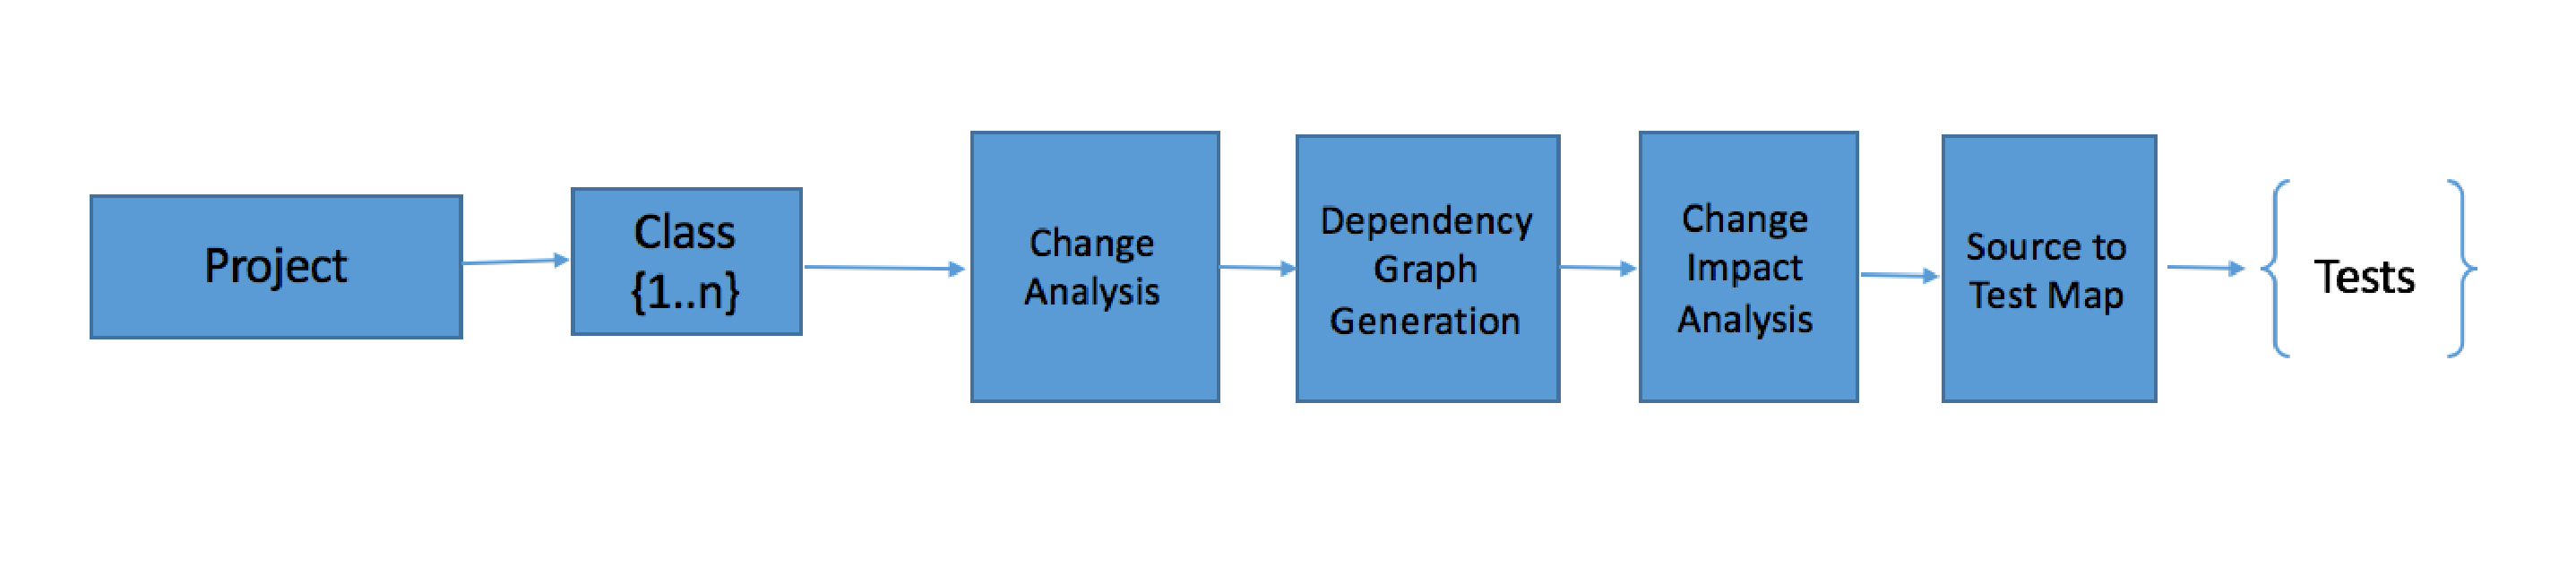
\includegraphics[width=0.99\linewidth]{pipe_1}%
        \hfill
        \caption{Sequential RTS pipeline}
    \end{subfigure}
    \vskip\baselineskip
    \begin{subfigure}[b]{\textwidth}
    \label{fig:sub2}
        \centering
        \includegraphics[width=0.99\linewidth]{pipe_2}%
        \hfill
        \caption{Parallel RTS pipeline}
    \end{subfigure}
    \caption{Generic pipeline of regression test selection.}
\end{figure}


\section{Example}
Table~\ref{comparison} summarizes the similarities and differences among four recent techniques, as well as our own, i.e., TLDR. What follows is an explanation of this table, followed by one concrete example of how three of these tools behave in the presence of a given change.

\begin{table}[b]
\centering
  \caption{Categorization of RTS Tools}
  \label{comparisontools}
  \resizebox{\columnwidth}{!}{%
    \begin{tabular}{|l|c|c|c|}
        \hline
    {\textbf{Technique}} &  \textbf{Granularity of} &  \textbf{Granularity of} &  \textbf{Dependency}\\
                         & \textbf{Test Selection} & \textbf{Change Analysis} &  \textbf{Collection} \\
    \hline
    \textbf{Ekstazi} \cite{ekstazi} & Class & File & Dynamic \\
    \textbf{STARTS} \cite{starts} & Class & Class & Static \\
    \textbf{HyRTS} \cite{hyrts} & Class/Method & Class/Method & Static+Dynamic\\
    \textbf{FaultTracer} \cite{faulttracer} & Method & Statement & Dynamic \\
    \textbf{TLDR } & Method & Member & Static \\
    \hline
    \end{tabular}%
    }
\end{table}%

Below, we explain the functionality of TLDR compared Ekstazi, STARTS, and HyRTS to illustrate how these three approaches differ along the dimensions of Table~\ref{comparison}. Table~\ref{example} shows an example Java project. Column \textit{Source} shows the source code and column \textit{Test} shows the test suite of the project. For each method in the source code, there is a test method in the test suite. Class \texttt{A} is extended by classes \texttt{B, D} and class \texttt{B} is extended by class \texttt{C}. Each of the sub-classes overrides method \texttt{A.f2}. Method \texttt{A.f1} is overridden by \texttt{C} and \texttt{D}. 

\begin{table*}
{\fontsize{12pt}{12pt}\selectfont
\centering
\caption{An Example Java Project}
\begin{tabular}{|p{0.5\linewidth}|p{0.5\linewidth}|}
\hline
\textbf{Source} & \textbf{Tests}  \\
\hline
\begin{lstlisting} [caption={}]
class A {
  String f1() { return new B().m1() + "a";}
  String f2() { return "a1";}
}
class B extends A {
  String m1() { return "b";}
  String f2() { return "b1";}
}
class C extends B {
  String f1(){ return super.f1() + "c";}
  String f2(){ return "c";}
}
class D extends A {
  String f1(){ return "d";}
  String f2(){ return "d";}
}
\end{lstlisting}

& 
\begin{lstlisting} [caption={}]
class TestA {
    A obj = new A();
    void tF1(){ assert(obj.f1() != null);}
    void tF2(){assert(obj.f2() != null);}}
class TestB {
    B obj = new B();
    void tM1(){assert(obj.m1() != null);} 
    void tf2(){assert(obj.f2() != null);}}
class TestC {
    C obj = new C();
    void tF1(){assert(obj.f1() != null);}
    void tF2(){assert(obj.f2() != null);} 
class TestD {
    A obj = new D(); // <--- note the declaration as A
    void tF1(){assert(obj.f1() != null);}
    void tF2(){assert(obj.f2() != null);}
\end{lstlisting}
\\
\hline
\end{tabular}
\label{example}
}
\end{table*}

The test selection sets when method \texttt{B.m1} changes are: 
\begin{itemize}
	\item Ekstazi: all test methods in \texttt{TestA, TestB}, and \texttt{TestC} -- 6 tests.
	
	\item STARTS: all test methods in \texttt{TestA, TestB, TestC}, and \texttt{TestD} -- 8 tests.
	
	\item HyRTS: test methods \texttt{TestB.tM1, TestA.tF1, TestC.tF1} -- 3 tests.
	
	\item TLDR: test methods that reach, or might reach, \texttt{B.m1}, specifically \texttt{TestB.tM1, TestA.tF1, TestC.tF1}, and \texttt{D.tF1} -- 4 tests.
\end{itemize}

Both Ekstazi and STARTS select tests at class level, so if any one test method needs to be retested, the entire class where that method is declared will be retested. TLDR selects tests at individual method level, so it can be more precise, as this example shows -- 4 test methods instead of 6 (Ekstazi) or 8 (STARTS). However, since this is an atomic change within the class, HyRTS only selects 3 methods. STARTS and TLDR use static analysis for tracking dependencies, while Ekstazi and HyRTS use dynamic analysis. Therefore, Ekstazi and HyRTS are more precise with respect to inheritance and method overriding. Let's look at the consequences of static vs. dynamic analysis for the test method \texttt{TestD.tF1}. That method instantiates a \texttt{D} object, but statically declares it as type \texttt{A}. Being an instance of \texttt{D}, and given that \texttt{D} overrides \texttt{A.f1}, the test method \texttt{TestD.tF1} does not need to be selected when \texttt{A.f1} changes. In this case, Ekstazi is able to identify that the \texttt{A}-object created in \texttt{TestD.tF1} is an instance of subclass \texttt{D}, while both STARTS and TLDR are unable to do so. 

Now let us consider another scenario where \texttt{Class D} is made to extend \texttt{Class C} but no method is changed. The test selection sets for this change are: 
\begin{itemize}
	\item Ekstazi: all test methods in \texttt{TestD} -- 2 tests.
	
	\item STARTS: all test methods in \texttt{TestA, TestD}, and \texttt{TestD} -- 4 tests.
	
	\item HyRTS: test methods \texttt{TestD} -- 2 tests.
	
	\item TLDR: No test method is selected -- 0 tests.
\end{itemize}

Even if no method was changed, \texttt{ClassD} will have different checksum, therefore, Ekstazi will select \texttt{TestD} and STARTS will select \texttt{TestA, TestD}. HyRTS considers class hierarchy change as class header change, thus it will perform file-level analysis and test selection. Therefore, it will select \texttt{TestD}. However, TLDR detects that even though the class hierarchy has been modified, no method was updated. Therefore, it will not select any test method. 
\chapter{TLDR Design and Implementation}
\label{sec:Implementation}

In this section, we discuss the design and implementation of TLDR. We first discuss the main algorithms of TLDR, and show how they can be parallelized. Then we describe the architecture of the implementation and each module in detail. 

\section{Test Selection and Dependency Extraction}

Algorithm \ref{tldr} describes the test selection algorithm underlying TLDR. The procedure takes two versions of a project as input -- $project_{n}$ and $project_{n-1}$ -- and returns the set of selected tests, $selected$. It does so by iterating through all class files of the latest version, checking for new, modified, and deleted ones. For new and modified classes, it then iterates through their declared members (methods and fields), checking for new, modified, and deleted members. For new and modified members, it extracts their static dependencies -- an algorithm explained next. Changes in classes and members are calculated by the checksum of their corresponding byte code using \textit{BLAKE2B}~\cite{aumasson2013blake2}, an efficient checksum algorithm. 

After updating the dependency graph, algorithm \ref{tldr} then generates $goldset$, which is a set of all members that may have indirectly been affected by changes in $project_{n-1}$, by performing a depth-first search (DFS) over the dependency graph (line 30 of the algorithm). Each method or field in $goldset$ is mapped to one or more tests that have dependencies on those entities. Test methods may have dependencies on other test methods and fields. Therefore, in order to select all impacted tests, transitive dependents of each test method in $mapped$ are collected. Finally, the set of tests, $selected$, is generated by another DFS in the dependency graph, but this time only traversing test-test dependency edges. 

\begin{algorithm}
{\fontsize{12pt}{12pt}\selectfont
\caption{Test Selection pseudo-code}
  \label{tldr}
  \begin{algorithmic}[1]
\Function{TLDR}{$project_{n}, project_{n-1}$}
\State $new, changed, goldset, mapped, selected \Leftarrow \phi$

\ForAll{\colorbox{blue!30}{$file_{n} \in project_{n}$}}
    \If{$file_{n} \notin project_{n-1}$}
        \State $\textit{insert}(file_{n}, \textit{blk2b}(file_{n}))$
    \EndIf
    \If{$\textit{blk2b}(file_{n})\neq\textit{blk2b}(file_{n-1})$} 
      \State $\textit{update}(file_{n}, \textit{blk2b}(file_{n}))$
      \ForAll{\colorbox{blue!30}{$member_{n} \in file_{n}$}}
           \State $extract = false$
          \If{$member_{n} \notin project_{n-1}$}
                \State $\textit{insert}(member_{n},  \textit{blk2b}(member_{n}))$
                \State $new = new \cup \{member_{n}\}$ 
                \State $extract = true$
          \ElsIf{$\textit{blk2b}(member_{n})\neq\textit{blk2b}(member_{n-1})$}
                 \State $\textit{update}(member_{n}, \textit{blk2b}(member_{n}))$
                 \State $changed = changed \cup \{member_{n}\}$ 
                 \State $extract = true$
          \EndIf
          \If{$extract\land isMethod(member_n)$ } 
                    \State $DEPEXTRACTION(member_{n})$
          \EndIf
          
          \ForAll{$member_{n-1} \in project_{n-1} - project_{n}$}
               \State $remove(member_{n-1})$
            \EndFor    
            
       \EndFor
    \EndIf
\EndFor

\ForAll{\colorbox{blue!30}{$member \in new \cup changed$}}
        \State $goldset = goldset \cup \textit{dfs(member)}$ 
\EndFor

\ForAll{\colorbox{blue!30}{$member \in goldset$}}
        \State $mapped = mapped \cup \textit{testmap(member)}$ 
\EndFor

\ForAll{\colorbox{blue!30}{$test \in mapped$}}
        \State $selected = selected \cup \textit{dfs(test)}$ 
\EndFor\\
\Return ${selected}$
\EndFunction
\end{algorithmic}
}
\end{algorithm}



\begin{algorithm}
{\fontsize{12pt}{12pt}\selectfont

\caption{Dependency Extraction pseudo-code}
  \label{dependency}
  \begin{algorithmic}[1]

\Function{DEPEXTRACTION}{$entity$}

\State $direct \Leftarrow $\{ $"putstatic"$, $"putfield"$, $"getstatic"$, $"getfield"$\}
\State $polymorphic \Leftarrow $\{$"invokevirtual"$, $"invokeinterface"$, $"invokestatic"$, $"invokespecial"$\}
\State $dependencies \Leftarrow \phi$\\

\LineComment[1\dimexpr\algorithmicindent]{Extract dependencies from method bytecode}
\ForAll{$instruction \in entity.bytecode$}
     \If{$instruction.type \in (direct \cup polymorphic) $}
         \State $dependencies = dependencies \cup instruction.callee$ 
     \EndIf
\EndFor
\ForAll{$member \in dependencies$}
    \If{$\textit{dep\_type(entity, member)} \in direct$}
        \State $ \textit{insert\_in\_db(entity, member)}$
    \ElsIf{$\textit{dep\_type(entity, member)} \in polymorphic$}
        \State $hierarchy \Leftarrow classHierarchy(member)$
        \If{$isOverridden(member, hierarchy)$}
            \State $nodes \Leftarrow getOverrides(member, hierarchy)$ 
        \ElsIf{$isMissing(member, class(member))$}
            \State $nodes \Leftarrow getInherited(member, hierarchy)$ 
        \EndIf
        \ForAll{$e \in nodes$}
        \State $ \textit{insert\_in\_db(entity, e)}$
        \EndFor
    \EndIf
\EndFor

\EndFunction
\end{algorithmic}
}
\end{algorithm}
\medskip

For each changed or new $file$, Algorithm~\ref{tldr} finds all new and changed members, and updates the dependency graph of changed methods by calling Algorithm~\ref{dependency}, our dependency extraction algorithm. This algorithm takes a method that has been changed and updates the global dependency graph by processing the bytecode of that method looking for instructions that establish dependencies to other methods and fields. Those dependencies may be direct (e.g. {\em putfield} establishes a dependency to the immediate target of the invocation) or indirect, which may involve polymorphic relations (e.g. {\em invokevirtual} involves dynamic dispatch, meaning that the exact type of the target is only known at runtime). Since JVM specification allows static methods to be polymorphic as well, we consider  {\em invokestatic} as polymorphic method invocation as well. In the case of a polymorphic target, we conservatively traverse the class hierarchy of that target either up or down, in search of all possible polymorphisms. For example, when the target is a method that is overridden in one or more subclasses of its class, we include all those overridden methods as dependencies, because we don't know the exact method that will be called at runtime; similarly, when the target is missing the method, it means that the method is inherited from a superclass. In this case, we have to traverse up in the class hierarchy and include the superclass method as a dependency.

\section{Safety}
An RTS technique is {\em safe} iff it selects all tests that are impacted by a change in the projects' files~\cite{willmor2005safe}. As currently implemented, TLDR is not entirely safe, because it does not track dependencies resulting from (a) the use of Java reflection, and (b) the use of external jars. This is not an inherent problem of TLDR; it is simply a limitation of its current implementation, which we plan to improve. This limitation affects other RTS tools that are based on static analysis~\cite{starts, hyrts, rtsplusplus}. TLDR is safe for all other cases, i.e. for {\em all} changes in the {\em source files} of the projects, as long as they don't involve reflection. 
In broad strokes, an RTS technique is safe when (1) it correctly captures all dependencies of all code entities down to the desired level of granularity; (2) it correctly slices the dependency graph for the set of entities that change from a version to another; and (3) it correctly identifies the tests that reach any part of those slices. For performance purposes, and as explained above, TLDR uses a static dependency graph. Because of dynamic dispatch, static analysis of object-oriented programs needs to take inheritance relations into account. Algorithm~\ref{dependency} describes the construction of this static extended dependency graph, which is complete, with the two exceptions: reflection and external jars. While constructing the static extended call dependency graph, it considers both direct (line (12)) and polymorphic (line (14)) dependencies.  

\section{Parallelism in TLDR}

The algorithms described above are not particularly new -- similar techniques for change analysis were used by other RTS tools~\cite{faulttracer, hyrts, ekstazi, starts}. However, in TLDR, we leverage the potential that Algorithm~\ref{tldr} has for parallelism to reduce test selection overhead. Specifically, instead of sequentially executing the entire algorithm, we parallelize lines (3), (9), (29), (32), and (35) -- these are portions of the algorithm that map certain processing functions to potentially large numbers of classes and their members.

\begin{figure*}
\begin{center}
  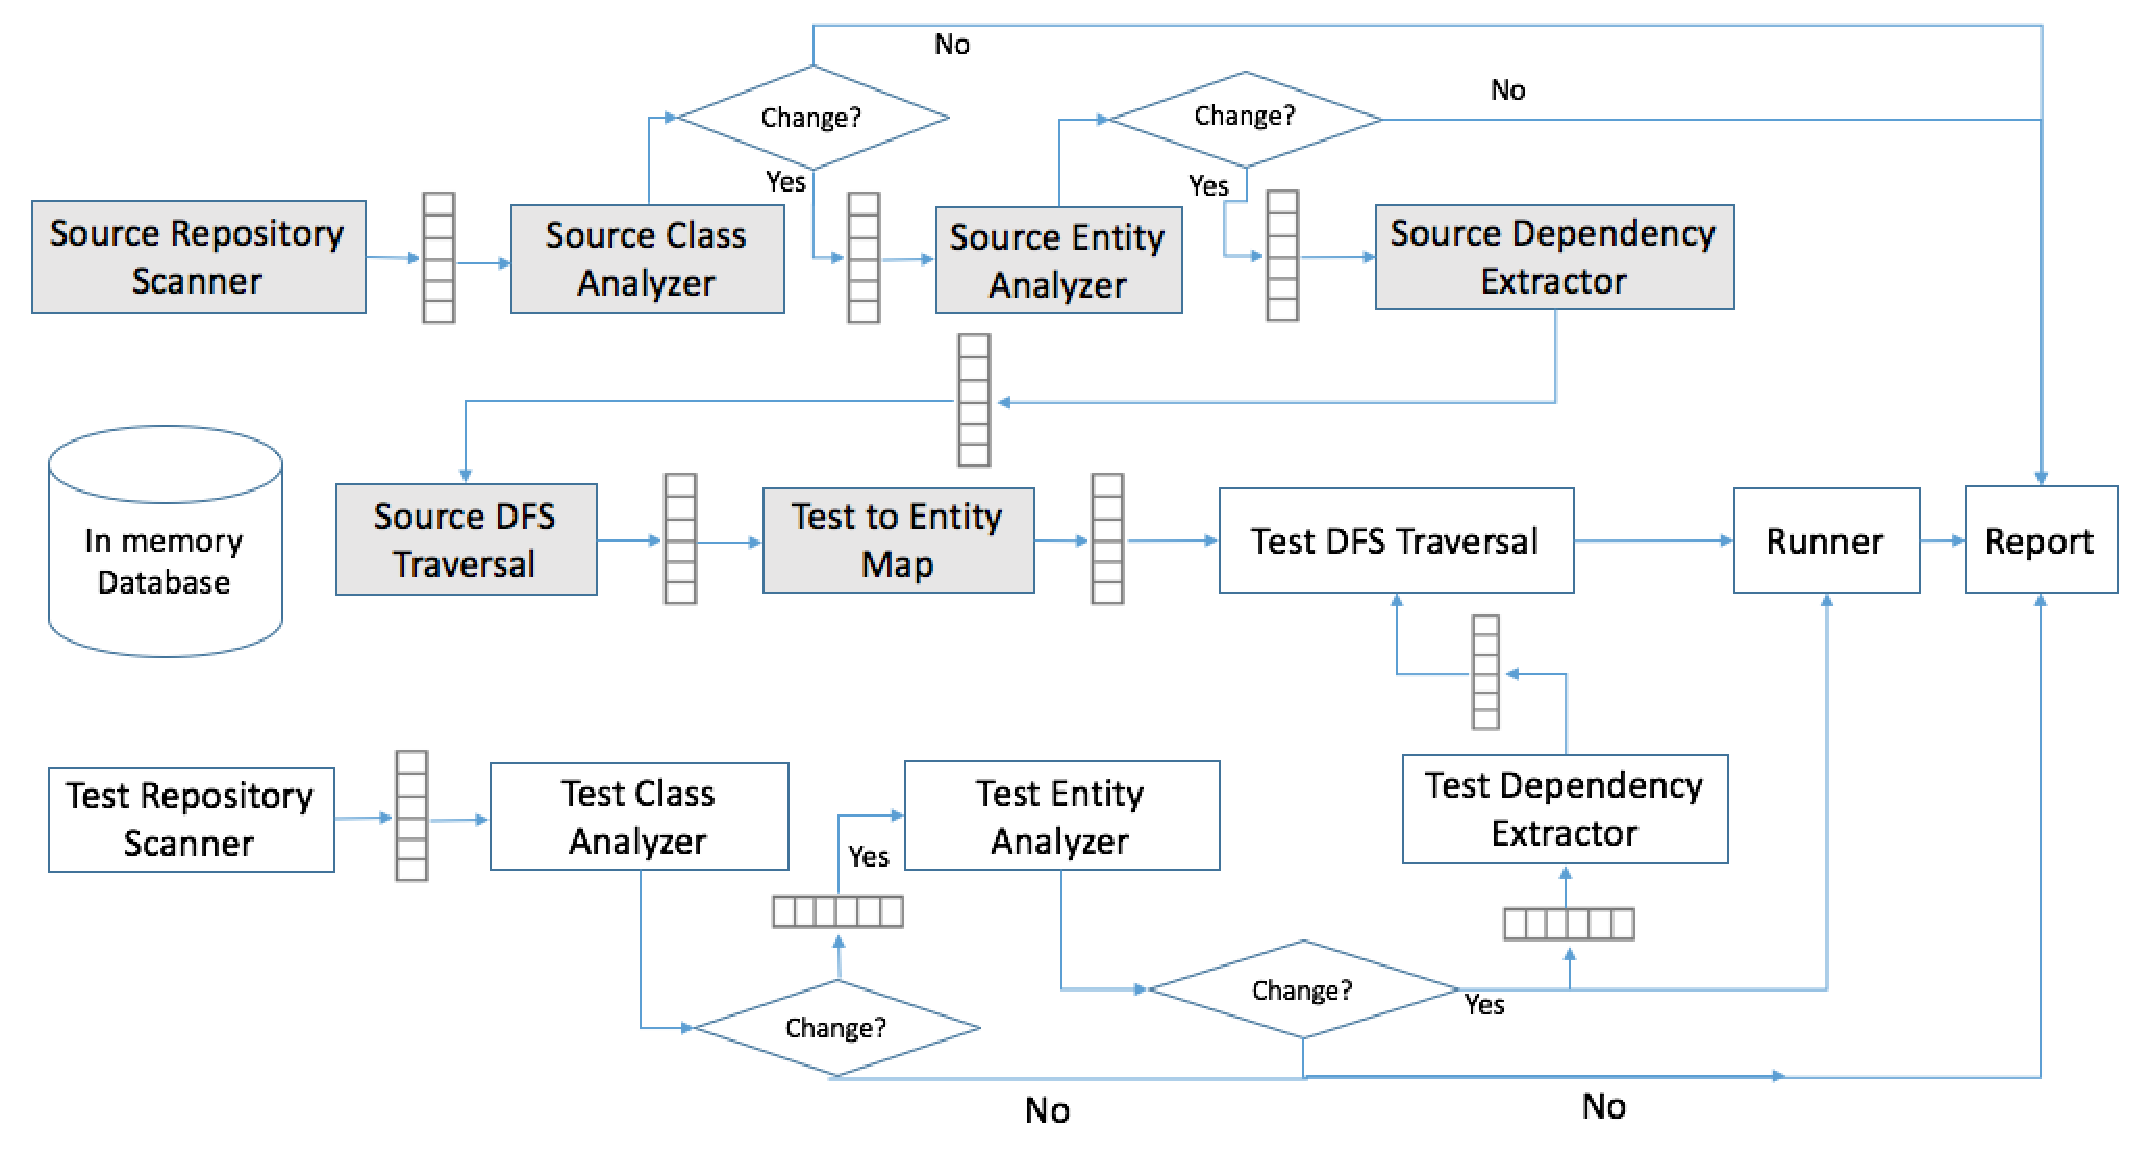
\includegraphics[width=18cm,height=8.5cm]{arch}
  \caption{Pipe-and-filter architecture of TLDR. The architecture contains two partially-independent pipelines, one for the source-code (marked as grey) and one for the test-code (marked as white).}
  \label{fig:tldr}
\end{center}
%\vspace{-5ex}
\end{figure*}

Figure \ref{fig:tldr} depicts the pipe-and-filter architecture of TLDR, which fully leverages parallelism for test selection and implements Algorithm~\ref{tldr}. The data elements of the pipeline are the absolute paths of the class files -- and the fully qualified name of the classes, methods, and fields. The pipeline takes as input the absolute path of each class file and outputs a set of selected tests. Components in the pipeline are multi-threaded and interact with each other through queues. The number of worker threads between two components is configurable, so to better take advantage of the hardware. As a result, TLDR can use the full computational power of each machine where it runs. 

TLDR's architecture contains two sub-pipelines: one associated with the source code under test -- which we refer to as the \textit{source pipeline} and whose constituent components are colored in grey -- and another associated with test code of the project -- which we refer to as the \textit{test pipeline} and whose constituent components are filled in white. These two pipelines operate in parallel and either asynchronously or synchronously, depending on which component is currently operating. Broadly, each of these two sub-pipelines has the following four components in common: \textit{Repository Scanner, Class File Analyzer, Entity Analyzer, Dependency Extractor}. Ultimately, these two sub-pipelines merge in the \textit{Test DFS Traversal} component, followed by execution of tests by the \textit{Runner} module. In the remainder of this section, we describe the functionality of each component.  

\section{In-Memory Database}
Deductive databases are often used to store program information as relations for numerous program analyses~\cite{lam2005context}. Similar to other RTS tools, we store program-specific information for incremental change analysis, dependency graph traversals, and mapping entities to a test method~\cite{faulttracer, hyrts, starts, ekstazi, legunsen2016extensive}. 

Data storage and retrieval are expensive processes. If nothing changes in the project, TLDR at a minimum needs to retrieve previously stored checksums of each class file for \textit{change impact analysis}, i.e. determining the entities affected by a change to another entity. Therefore, performance of RTS greatly depends on the database schema as well as storage technology.  To achieve high performance, we use an in-memory database server, \textit{Redis}. We implemented a customized \textit{database handler} which is available to all the components in the pipeline. The database handler provides thread-safe APIs to read, update, and delete values.

\begin{table}
  \scriptsize
  \centering
  \caption{Hashtables used by TLDR's In-Memory Database}
    \begin{tabular}{r | ll}
    \multicolumn{1}{l|}{\textbf{Hashtable No.}}  & \textbf{Key} & \textbf{Value} \\
    \hline
    1     & class absolute path & checksum \\
    2     & FQN of entity & checksum \\
    3     & FQN of entity & set of FQN of dependent entity \\
    4     & FQN of entity & set of FQN of dependency entity \\
    5     & FQN of Class & set of FQN of super class and interfaces \\
    6     & FQN of Class & set of FQN of the subclasses \\
    7     & FQN of entity & set FQN of test methods \\
    8     & FQN of test entity & Boolean \\
    \hline
    \end{tabular}%
  \label{tab:hashtables}%
\end{table}


\vspace*{0.2cm}
\noindent

Conceptually, Redis tables are hashtables, i.e. key-value pairs. In TLDR, the keys are the fully qualified name (FQN) of the entities and the values are either a hashcode, i.e. checksum, or a set of FQNs. Table \ref{tab:hashtables} shows the 8 hashtables used by TLDR, each identified with a table ID. Hashtable 1 and 2 store the checksum of each file and entity i.e. field and method respectively. These two hashtables used for change analysis. Hashtable 3 stores the set of dependents of each field and method. This table is the dependency graph of the project. It is used by the DFS algorithm to traverse the firewall of each changed field and method. Hashtable 4 is the inverse of hashtable 3. It stores the set of dependencies of each field and method. This table is needed for faster update of hashtable 3 when a method is no longer another method's or a field's dependent. Hashtable 5 stores class-hierarchy information. This table is used by algorithm \ref{dependency} to construct polymorphic edges in the dependency graph. Hashtable 6 is the inverse of hashtable 5 and facilitates faster update of hashtable 5 when the class hierarchy of the projects changes. Hashtable 7 stores entity to test mapping information. This is used in mapping tests to each field and method in $goldset$ in algorithm \ref{tldr}. Hashtable 8, stores all test methods and fields. This table is used along with table 3 to traverse within the test suite. 


\section{Repository Scanner}

\noindent
Both the source and test pipelines start by scanning the repository of the project using a recursive depth-first search algorithm that locates all class files in the repository. In a Maven project, source classes reside on \textit{*/target/classes/} directory and test classes reside on \textit{*/target/test-classes/} directory. Source Repository Scanner collects all source classes and Test Repository Scanner collects all test classes from the above-mentioned directories respectively. A Maven project can be hierarchical with multiple modules. Each module can have its own independent source and test directory. Each Repository Scanner can discover all such source and test directories. 

\section{ Class Analyzer and Entity Analyzer}

TLDR performs change impact analysis during two subsequent stages: one for the class level and another for the method- and field-level. TLDR analyzes change at the bytecode level. We choose this level because many changes that do not affect tests can be filtered out when analyzing bytecode but would result in unnecessary test selection at the source code level. For instance, new or changed comments or equivalent code at the statement level (e.g., \textit{var++} instead of \textit{var = var + 1}), etc. yields the same checksum. Previous testing approaches have followed a similar practice~\cite{ekstazi, hyrts, starts, xu2007regression, fraser2011evosuite}. 

Broadly, TLDR can detect 16 types of changes, shown in Table \ref{tab:changes}. Altogether, these 16 change types cover a wide variety of possible changes in object-oriented languages and at least the same type of changes handled by state-of-the-art RTS techniques \cite{ekstazi, hyrts, starts}.

\begin{table}
  \scriptsize
  \centering
  \caption{Changes detected by TLDR}
    \begin{tabular}{r | ll}
    \multicolumn{1}{l|}{\textbf{}}  & \textbf{Type of Change} \\
    \hline
    1     & Addition of a new class \\
    2     & Addition of a new method \\
    3     & Addition of a new field \\
    4     & Addition of a new static initializer \\
    5     & Change of a method definition \\
    6     & Change of a field value\\
    7     & Change of the class hierarchy \\
    8     & Change of a class signature \\
    9     & Change of a field signature \\ 
    10    & Change of a method signature \\ 
    11    & Change of a static initializer \\ 
    12    & Deletion of a class \\ 
    13    & Deletion of a method \\ 
    14    & Deletion of a field \\ 
    15    & Deletion of a test case \\
    16    & Deletion of a static initializer \\
    \hline
    \end{tabular}%
  \label{tab:changes}%
\end{table}%

TLDR uses a 16 character-long alpha-numeric checksum as part of its change impact analysis. The efficiency of the test selection pipelines also depends on checksum calculation. To maximize efficiency of checksum usage, TLDR uses \textit{BLAKE2B}~\cite{aumasson2013blake2}, which is 4 to 8 times faster than \textit{SHA256, BLAKE, and SHA-1}. 

For each \textit{Class File Analyzer}, i.e., source and test, TLDR calculates the checksum of bytecode. Only the class files whose checksums are different than the previously computed value are forwarded to the next component in the pipeline for field- and method-level change analysis as shown in figure\ref{fig:change_class}. 

\begin{figure*}
\begin{center}
  \includegraphics[width=14cm,height=6.5cm]{redis}
  \caption{Change analysis of class files. Only the changed class files are passed to the next module.}
  \label{fig:change_class}
\end{center}
\end{figure*}

For both source and test \textit{Entity Analyzer} components, TLDR splits the class file into methods and fields using \textit{Apache Common BCEL} library. The checksum is calculated by concatenating the entity's (i.e., method's or field's) modifier, signature, and body. We omit \textit{StackMap Table} of the methods. The offset delta of StackMap of a method depends on the overall offset of the class file. Addition or deletion of a statement in the preceding method can possibly change the offset information of the subsequent methods' StackMap Table. This can cause changes in the checksum of a method even though that method did not change in code. 


\begin{figure*}
\begin{center}
  \includegraphics[width=16cm,height=7.5cm]{class}
  \caption{Change analysis of methods and fields. Each changed class file is split into methods and fields and fed to the change analysis module.}
  \label{fig:change_method}
\end{center}
\end{figure*}


For fields, we calculate the checksum of the signature of the field. In addition to change analysis, we perform three tasks in Entity Analyzer: (1) extracting the class-hierarchy information, i.e., super-class and interfaces of the class; (2) update the class-hierarchy information in the database if the class hierarchy is changed; (3) update and sync the dependency information if a method or field has been deleted. 

\section{ Dependency Extractor}

\noindent
Algorithm \ref{dependency} implements Dependency Extractor. For each method including constructors (\texttt{<init>}) and static initializer (\texttt{<clinit>}), both source and test, we extract dependencies by parsing the operands of the following 13 bytecode instructions: i) \texttt{invokestatic}, ii) \texttt{invokespecial}, iii) \texttt{invokevirtual}, iv) \texttt{invokeinterface}, v) \texttt{getstatic}, vi) \texttt{getfield}, vii) \texttt{putstatic}, viii) \texttt{putfield}, ix) \texttt{checkcast}. For \texttt{invokevirtual}, \texttt{invokeinterface}, \texttt{invokestatic}, and \texttt{invokespecial} we retrieve all overridden versions of the dependency method by traversing the class hierarchy. 

The extracted dependency information is inserted in both a forward and inverted index of dependencies. The inverted index is being used to formulate the transitive dependents of the changed methods, while the forward index is being used to update and synchronize the database in case a dependency is deleted in a particular revision. For the test pipeline, dependency information is indexed into two tables: (1) Hashtable 3 and (2) Hashtable 7. Test dependencies on source methods are used to map a source entity to a test method. Test methods have dependencies to other test members. To select all impacted test methods, we have to find the transitive dependents of each test that mapped to a method or field in $goldset$. 

%Test dependencies to other test methods are used to traverse the transitive dependencies among test methods. Data from this module is forwarded to the DFS Traversal Component for subsequent analysis. 

\vspace*{0.2cm}
\noindent
\subsection{ DFS Component}

\noindent
This component is a Depth-first search algorithm that traverses the transitive dependency of each changed or newly added entity. DFS Traversal of the source pipeline is synchronized with the Dependency Extractor of the test pipeline. Algorithm \ref{tldr} waits for Test Dependency Extractor to finish for all data elements in the test pipeline before forwarding each member in $goldset$ to Test to Entity Map component. This is because in order to map the source members to test methods, all test methods must be parsed and their updated dependency to the source methods must be indexed. Source DFS Component collects the firewall of each changed or new member. 

The DFS component of the test pipeline gets input from both Test Dependency Extractor of the test pipeline and Test to Entity Map component of the source pipeline. This module is the meeting point of the two sub-pipelines. Test methods might have dependencies on other test fields, parameterized test methods, or helper methods. Test DFS component allows traversing these transitive dependencies for each new or mapped test method. This component is customized to traverse transitive dependency within the test suite.


\section{Test to Entity Map}

This component is only present in the source pipeline. This is a mapping function that maps each entity in the transitive dependent set of each changed or newly added method and field to a test method, i.e., a test method which has a direct dependency on one or more entities in the transitive dependent set. Mapped tests are then forwarded to test DFS Traversal to form a transitive set of impacted changed methods. 

\section{Runner}

TLDR extends \texttt{Maven SureFire} which is a plugin to run JUnit tests in Maven projects. TLDR runs the only the selected tests by dynamically updating the \texttt{test} field of \texttt{SureFire} by Java instrumentation. In order to run the selected tests parallelly, TLDR updates \texttt{SureFire} configuration values -- \texttt{forkCount} and \texttt{reuseForks}. These flags enable Surefire to spawn a specified number of JVM processes and distribute test run load among the processes parallelly.


\section{TLDR Artifact}

TLDR is an open-source project. TLDR's source-code can be found in this GitHub repository : \href{url}{http://www.github.com/Mondego/TLDR}. The tool has not been released in the Maven Central Repository yet. Therefore, it needs to be installed in the local maven repository. To do so, the source-code needs to be cloned into the local machine and within the repository, the following maven command is needed to be executed \textit{mvn clean compile install}. After installing TLDR in the local maven repository, the following XML snippet needs to be added in the \textit{<plugins>} block of the \textit{pom.xml} file of the project which is to be tested through TLDR. 
\newline
\begin{lstlisting}
<plugin>
	<groupId> com.mondego.ics.uci </groupId>
	<artifactId> tldr-plugin </artifactId>
	<version> 1.0.2-SNAPSHOT </version>
	<configuration>
		<goalPrefix> tldr </goalPrefix>
		<skipErrorNoDescriptorsFound> true </skipErrorNoDescriptorsFound>
	</configuration>				
</plugin>
\end{lstlisting}

Before running the plugin, a Redis server must be started locally. Finally, the following command should be executed - 
\textit{mvn com.mondego.ics.uci:tldr-plugin:1.0.2-SNAPSHOT:tldr -Dmultimodule.projectname=<project-name>}. This will invoke Maven surefire and the test report will be placed inside the \textit{Target} folder of the repository. TLDR provides several optional command-line options. Some relevant command-line options are as follows -

\begin{itemize}
    \item -Ddebug.flag: turns on the debug prints during different stages of the pipeline. 
    \item -Dlog.directory: specifies the location of log files that are generated during analysis and testing.  
    \item -Dcommit.hash: specifies the hashcode of a particular commit on which TLDR is to be run.
    \item -Dcommit.serial: specifies the serial number of the project iteration. This flag is useful in iterative evaluation of TLDR.
    \item -Dfork.count: specifies the number of process forks test runner should use. 
    \item -Dthread.count: specifies the number of threads the test runner should use. 
 \end{itemize}

\chapter{Safety of TLDR}
\label{sec:Implementation}

\section{Safety of TLDR}

An RTS technique is {\em safe} iff it selects all tests that are impacted by a change in the projects' files. As currently implemented, TLDR is not entirely safe, because it does not track dependencies resulting from (a) the use of Java reflection, and (b) the use of external jars. This is not an inherent problem of TLDR; it is simply a limitation of its current implementation, which we plan to improve. TLDR is safe for all other cases, i.e. for {\em all} changes in the {\em source files} of the projects, as long as they don't involve reflection. 

In broad strokes, an RTS technique is safe when (1) it correctly captures all dependencies of all code entities down to the desired level of granularity; (2) it correctly slices the dependency graph for the set of entities that change from a version to another; and (3) it correctly identifies the tests that reach any part of those slices. We use the concept of \textit{Static Extended Dependency Graph} to capture (1), and the concept of \textit{Firewall} to capture (2).

\subsection{Static Extended Dependency Graph}

Zhang et al. presented extended dependency graphs for RTS tools~\cite{b37} in the context of dynamic dependency tracking. Extended dependency graphs model methods and fields as vertices in the graph, and the edges are the dependencies. 
For a set of methods, $M$ and a set of fields, $F$, extended dependency graph, $G$ in an OO language is defined as follows~\cite{b38}: 
\begin{definition}
Dynamic Extended Dependency Graph: $G = <V, E>$ where $ V = M \cup F$ and $E = <v, v'>$ where $v \in M, v' \in \textit{calledBy}(v) \land V$  
\end{definition}
In this definition $calledBy(v)$ denotes the set of members (methods or fields) that the method $v$ refers to at runtime. It is worth noting that $G$ is dynamic in nature. This means $G$ has edges that correspond to dependencies among members that are resolved at runtime. 
For performance purposes, and as explained before, TLDR uses a static dependency graph. Because of dynamic dispatch, static analysis of object-oriented programs needs to take inheritance relations into account. Algorithm~\ref{dependency} describes the construction of the static extended dependency graph. Formally, we define the static extended dependency graph $SG$ as follows:

\begin{definition}
\label{def:staticextendedcallgraph}
Static Extended Dependency Graph: 
\end{definition}
\noindent
$SG$ = $(V, E)$ where $ V = M \cup F$, $E$ = $(v, v')$ where $v \in M$, $v' \in V \land (\textit{referencedBy(v)}  \cup (overridden(referencedBy(v)) \lor inherited(referencedBy(v)) ))$  

In the definition, $E$ is the set of edges (dependencies) that are direct or indirect via polymorphism. $referencedBy(w)$ is  the set of members that method $w$ calls or refers to. $overridden(w)$ is the set of all methods that override method $w$, and $inheritedBy(w)$ is the set of methods inherited from superclasses. In Java, all the non-reflective dependencies among members can be captured by the following byte code instructions: \texttt{invokevirtual, invokeinterface, invokestatic, invokespecial, getstatic, getfield, putstatic, putfield}. $SG$ thus, includes all types of dependencies in Java bytecode, except reflective dependencies.  

\subsection{Firewall}

The concept of firewall in software testing was first discussed by White et al.~\cite{white1992firewall} and has since been adopted into object-oriented testing as well~\cite{white2003firewall, white2005utilization, white2008extended, starts, hyrts}. The firewall of a given code entity (i.e. file, class, method, field, or statement) is the set of entities that can be impacted by a change in that entity. Finding the firewall of a changed entity requires traversing transitive dependents of that entity. In a static RTS, such traversal involves traversing both direct and polymorphic edges. Class firewall has been proposed by Legunsen et al. for a static class-level RTS ~\cite{legunsen2016extensive}. A class-level RTS selects all test classes that have dependency on any class in the class firewall of a changed class. Similarly, a method-level RTS selects all test methods that have dependency on any method or field in the method or field firewall of a changed method or field. Formally, the firewall of a member in a static graph, $SG$ can be defined as follows: 
\begin{definition}\label{def:firewall}
Firewall: $F(w) = {\bigcup}_{\forall v}{DFS(v, SG)}, w \in M,v \in V \land calledBy(w) $
\end{definition}

In this definition, $DFS(v,SG)$ returns a set of members that are connected to node $v$ in a static graph $SG$. Definition \ref{def:firewall} defines firewall of a member as the union of firewall of all dependent members. 

\subsection{Proof of Safety of TLDR}
A safe static method-level RTS tool captures both static and polymorphic dependencies among fields and methods. To prove the safety of TLDR we need to prove that TLDR captures all types of dependency in Java bytecode i.e. creates a static extended dependency graph. Also, we need to prove that it collects all members that may be impacted by a given change in source code. Therefore, to prove the safety of TLDR, we prove that -- (1) TLDR constructs a static extended dependency graph $SG$ (2) TLDR selects all tests that map to $firewall(v)$ where $v$ is a changed entity. 

\begin{theorem}\label{theory}
TLDR constructs static extended dependency graph $SG$
\end{theorem}
\begin{proof}
Function $DEPEXTRACTION$ is being called for each changed or new $v \in M \cup F$. It takes the dependent entity $v$ and extracts the set of its direct dependencies, $dependency$. Let us consider that $DEPEXTRACTION$ only captures static edges. Line(13) inserts each $member \in dependency$ as $v$'s dependency with which $v$ has \texttt{invokestatic, invokespecial, getstatic, getfield, putfield, putstatic} relation. These are static edges. However, line (22) inserts the overridden and inherited versions of each $member$ with which $v$ has \texttt{invokeinterface, invokevirtual} relations. Since the edges are between the dependent and all the overridden and inherited versions of the dependency members, they are polymorphic edges according to ~\cite{sundaresan2000practical}. Contradiction. 

Therefore, $DEPEXTRACTION$ captures both static and polymorphic edges, thus according to definition \ref{def:staticextendedcallgraph} constructs $SG$.
\end{proof}



\begin{theorem}\label{theory}
TLDR selects all tests $t$ that has either direct or polymorphic dependency to $firewall(v)$ where $v$ is a changed entity. 
\end{theorem}
\begin{proof}
For a changed $v \in M \cup F$, let us assume algorithm \ref{tldr} returns a set of tests $selects$ that does not include one $t$ which has edge to a $v^{'} \in V \cup F$ and $v^{'} \in firewall(v)$. For each new and changed $v$, TLDR calls $DFS(v)$ on $SG$ created by $DEPEXTRACTION$. According to \cite{tarjan1972depth}, $DFS(v)$ returns a set of all entities reachable from $v$ in $SG$. Therefore, $DFS(v)$ returns $firewall(v)$. This set is included in $goldset$. Line (25) adds each $t$ that maps to any $v^{'} \in goldset$ in $mapped$. Each $t$ in $mapped$ is impacted by change in source code. Line (28), then calls $DFS(t)$ for each $t$ in mapped to collect all $t'$ that is impacted by $t$ and adds them to $select$.  Contradiction. Therefore, $select$ includes all test methods that map to $firewall(v)$ for each changed entity $v$.

\end{proof}

%Therefore, the technique used in TLDR is safe. 








\chapter{Evaluation}
\label{sec:evaluation}
In this chapter, we discuss the evaluation of TLDR. Regression test selection tools are primarily evaluated based on their precision and efficiency~\cite{ekstazi, hyrts, starts, faulttracer}. We evaluated TLDR in terms of the number of selected tests (precision) and end-to-end testing time (efficiency). As mentioned earlier, the baseline RTS techniques of our evaluation are Ekstazi, STARTS, and HyRTS. Before discussing the findings of our evaluation, we discuss our research questions, the projects that serve as subjects for our experiments, and the experiment setup. 

\section{Research Questions}
For our evaluation, we answer the following two research questions:  
\begin{enumerate}[leftmargin=2mm,itemindent=.5cm,labelwidth=\itemindent,align=left,noitemsep,topsep=0pt]
	\item \textbf{RQ1: To what extent does TLDR reduce the number of tests selected for re-execution compared to the baseline RTS techniques?}
	
	As demonstrated in the previous section, TDLR is safe for all changes in source files that do not involve reflection, similar to state-of-the-art approaches \cite{starts,ekstazi}. However, one of TLDR's goals is to maintain precision, i.e., select as few tests as possible for re-execution while still identifying all possible faults that the original test suite can reveal. We assess TLDR's ability to reduce tests selected while maintaining safety for this research question in contrast to the baselines.
	
	\item \textbf{RQ2: What is the end-to-end testing time of TLDR as compared to retest-all, and the baseline RTS techniques?}
	
	One major contribution of TLDR is to significantly reduce end-to-end testing time compared to the state-of-the-art techniques, i.e., Ekstazi, STARTS, HyRTS, re-running all the tests from the original test suite, i.e., retest-all, and re-running all the tests from the original test suite with parallelization. As a result, we evaluate each of these six techniques in terms of end-to-end testing time for our experiments.
\end{enumerate}

\section{Data Collection }

\begin{table}[htb]
\centering
  \caption{Meta-information of the study projects}
  \label{projectmeta}
  \resizebox{0.8\columnwidth}{!}{%
    \begin{tabular}{|l|r|r|r|r|r|}
        \hline
    {\textbf{Project}} & \textbf{\#Class} & \textbf{SLOC}  & \textbf{\#Tests} & \textbf{\#Commit } & \textbf{\#Star} \\
    \hline
    Asterisk-java &  839  & 111721 &   260   & 2004  & 340 \\
    Commons-dbutils &  96  & 14836  &  307    &  783 & 272 \\
    Commons-jxpath &  232  & 40128  &    386 &   601 & 150 \\
    Commons-validator &  150  & 33880 &  544   &   1543 & 127 \\
    Compile-testing &   49 &  10389 &   221  &   354 & 570 \\
    Invokebinder &  26  & 7878 &  99  &     163 & 95 \\
    Chronicle-Map &  453  & 59294 &   1036   &  2935 & 2200 \\
    Retrofit &  283  &  36610 &  694 &    1865  & 37900\\
    Logstash-encoder &  227  & 26682 &   320   &   829 & 1800 \\
    Jfreechart &   1022 & 283820 &  3182   &  4179 & 683 \\
    Commons Collections & 856   & 62858 &  2884  & 3094  & 347 \\
    Commons IO & 321   & 26882   & 1468  & 2158  & 574 \\
    Chronicle Map &     424  & 28697        &    665   & 2492  & 1648 \\
    Commons Cli & 58   & 12326   & 310  & 915  & 144 \\
    Joda Time & 530   & 86184   & 5332  & 2104  & 4036 \\
    Commons Email & 47   & 12474   & 209  & 839  & 60 \\
    Commons Fileupload &  64  & 10385   & 113  & 954  & 104 \\
    Commons Lang & 714   & 74934   & 3749  & 5434  & 1628 \\
    Commons Math & 1941  & 174505  & 6065  & 6402  & 263 \\
    Commons Pool & 179   & 14337   & 570   & 1908  & 245 \\
    
    \hline
    \end{tabular}%
    }
\end{table}%

We selected 20 open-source Java projects from GitHub to evaluate TLDR against the baselines. These projects were either single or multi-modular. These projects were used in the evaluation of prior RTS techniques~\cite{gligoric2015ekstazi,hyrts,starts,legunsen2016extensive}. TLDR's implementation supports Maven and JUnit 4.x but not other build automation tools or unit-testing frameworks. As a result, we excluded projects that had the following characteristics - 

(1) use Gradle, Ant, or other build tools and testing frameworks other than JUnit 4.x, 

(2) have test suites that could not be executed by either Ekstazi, STARTS, HyRTS, or TLDR. For example, running the test suite of \textit{Guava} caused our Java Virtual Machine to crash even after setting up the maximum heap size possible in our machine. While all large projects can be benefited from RTS tools, we excluded these projects due to resource and implementation limitations. Some projects had external environment dependencies, for example, database server, socket connection, etc. Therefore, those projects could not be run without externally setting up environment dependencies. For example, in order to execute the test suite of Apache Common Net, a WebSocket connection between two machines is needed to be established. 

(3) are active and popular. Projects' activity and liveliness are measured by the number of commits and popularity is measured by the number of stars. We excluded projects that had less than 500 commits and less than 50 stars. 

These project exclusion criteria enable a fairer and accurate comparison among the RTS techniques in our evaluation.

Table~\ref{projectmeta} shows the list of projects; project size in terms of number of classes, and source lines of code (SLOC); test-suite size in terms of number of test methods; and project metadata, i.e., number of commits and the number of stars in the latest commit from GitHub using~\textit{Sourcerer}~\cite{linstead2009sourcerer}, a static code analysis infrastructure. 

\section{Experiment Setup}

\begin{table}[htbp!]
\centering
\caption{Projects and Sampled Commits }
\label{hashcodes}
\resizebox{0.8\textwidth}{!}{
\begin{tabular}{|l|l|}
\hline
\textbf{Project Name} & \textbf{Commit Hash}\\
\hline

Asterisk-java &
44aee1b44afbb1e4dc518ad8ea32126291318c32 \\
Commons-cli &
De5f2b46fa952a69a8819b60d60a03eac1154282 \\
Commons-collections &
Fa11e5702bafb392b20633a0e8c9617cab9a0276 \\
Commons-dbutils &
2ed6a127bd830adbe2b385d9ee62ead2f0e61fc5 \\
Commons-email &
77ac7bcd01f558eaeeecf50e478e939d74293942\\
Commons-fileupload &
f4cab5702b6e7d6c019c9fec29357ad2b552783d\\
Commons-functor &
049e4fbdd987a405f2fcc1b97e6c7903db068965\\
Commons-jxpath &
07b898f72113be256ecc1420f5388261d951c547\\
Commons-math &
b95a43fa9af718899d03bbc2c10587c069c707f0\\
Commons-pool &
c9f61e36b119a824c6c02ee6009eddae47bfecef\\
Commons-validator &
dcf935a9ef9909e59f631ecbda6d00e2a8ac8450\\
Compile-testing &
7e2b01560666ba10b330f1984fdbb3251f2548a1\\
Invokebinder &
d539764d7ebb26edc5080a2ecd642d483bcb6030\\
Chronicle-Map &
857f544a26e21e169280089b5f8d24b3b880782f\\
Retrofit &
bf9f11430de52b13f2f3f1aa2be4b64d6471a46d\\
Commons-lang &
efbfd2de9765bc01e4916b16e8eb82370f25ff82\\
Commons-io &
724125eff6608884b0ac1c59f62695ecf43e5c8a\\
Joda-time &
7b549b1d9ad88be845e469222c57c144ae1b7da1\\
Logstash-encoder &
73437e6a3212985eeb55bcb9047c6def74161800\\
Jfreechart &
9d7887f00218d39b63f209e86e248f895b10cb87\\


\hline
\end{tabular}
}
\end{table}

For each project, we collected hashcodes for the latest 30 commits that compile from the git log of the corresponding projects. The sampled hashcodes are shown in table \ref{hashcodes}. For evaluating the RTS techniques, we installed TLDR, Ekstazi\footnote{collected from ~\textit{https://github.com/gliga/ekstazi}}, STARTS\footnote{collected from ~\textit{https://github.com/TestingResearchIllinois/starts}}, and in our local machine. HyRTS is not open-source. We collected the HyRTS artifact from the authors of the tool~\cite{hyrts}. STARTS had logs of test selection time and test runtime. For Ekstazi and HyRTS, we modified the plugin code to log test selection and run time individually at the end of test selection and test execution phase respectively. It should be noted that we did not modify any existing code, therefore, the core functionalities of these tools remained the same. We implemented a bash script to automatically run the experiment. For each project in our evaluation, the script retrieves the commit in the project's corresponding commit sequence $C'$, using the \texttt{git reset} command and each commit's corresponding hashcode. The script then uses Maven to clean out the project, compile its source code, and compile its test code without running it. Cleaning the project out before compiling it reduces any potential errors arising from residual files remaining in the project’s directories that were produced during previous runs of the project. Some projects had release audit plugin, for example, \textit{Apache Rat} and style formatting plugin, for example, \textit{Maven Checkstyle}. We turned these plugins off because, for some projects, they caused errors while running TLDR as well as the other three RTS plugins. 

For each commit, we ran the test once for each of the six techniques we evaluate, i.e., TLDR, Ekstazi, STARTS, HyRTS, retest-all, and parallel retest-all. To run parallel retest-all, we set \texttt{forkCount} and \texttt{reuseForks} flag of Maven Surefire so that it spawns a specified number of JVM processes concurrently to execute the tests. For our experiment, we used 8 JVM forks to run tests in parallel. Note that, TLDR's test runner also had 8 JVM forks. For each of these runs, we collected the test reports generated by \textit{Maven Surefire}. The generated report is in HTML format. We implemented our own parser to collect the number of tests run from the Surefire HTML reports and test selection and test execution time from the log files generated by our custom code. 

The experiment was conducted using a remote server with 256 GB (1867 MHz) DDR3 RAM, a 112-core \textit{Intel(R) Xenon(R) E5-4650} CPU, Linux 3.10.0 operating system, and 500G of solid-state disk. We used a local server of \textit{Redis 3.2.8} as our in-memory database. 




\begin{landscape}
\begin{table*}[htbp]
  \centering
  \caption{Number of tests run for Retest-All, Parallel Retest-All, TLDR, STARTS, Ekstazi, and HyRTS}
  \resizebox{1.32\textwidth}{.36\textwidth}{
    \begin{tabular}{|l|r|r|r|r|r|r|r|r|r|r|r|}
    \hline
     & \multicolumn{1}{|r|}{} &   \multicolumn{1}{|r|}{}     & \multicolumn{1}{|r|}{} & \multicolumn{2}{c|}{\textbf{TLDR}} & \multicolumn{2}{c|}{\textbf{STARTS}} & \multicolumn{2}{c|}{\textbf{Ekstazi}} &
     \multicolumn{2}{c|}{\textbf{HyRTS}} \\
   \cline{5-12}
   \multicolumn{1}{|c|}{\textbf{Project}} & \multicolumn{1}{|r|}{\textbf{Commit}} & \multicolumn{1}{|r|}{\textbf{$\sum Test_{all}$}} & \multicolumn{1}{|r|}{\textbf{$\sum Test_{par}$}} & \multicolumn{1}{r|}{\textbf{$\sum Test$}} & \textbf{$\%tests$} & \textbf{$\sum Test$} & \textbf{$\%tests$ } & \textbf{$\sum Test$} & \textbf{$\%tests$} & \textbf{$\sum Test$} & \textbf{$\%tests$}\\
    \hline
    
    
\multicolumn{1}{|l|}{asterisk-java}&	44aee1b	& 7771	& 7771	&1157	&14	&2121&	26	&1962&	24	&1877&	24 \\
\multicolumn{1}{|l|}{commons-cli}&	de5f2b4 &	12480&	12480&	615&	4	&1200&	8	&879&	6	&739&4 \\
\multicolumn{1}{|l|}{commons-collections}&	fa11e57	&749910&	749910	&23606	&2	&89161	&10	&36914&	4	&25746	&2\\
\multicolumn{1}{|l|}{commons-dbutils}&	2ed6a12	&9210&	9210&	512	&4	&1830	&18	&1142&	12	&925&	10 \\
\multicolumn{1}{|l|}{commons-email}&	77ac7bc	&5700	&5700	&245&	2&	1710	&30&	380	&6	&219	&2 \\
\multicolumn{1}{|l|}{commons-fileupload}&	f4cab57	&2760&	2760	&334&	12	&1622	&58	&1104	&40&	412	&14 \\
\multicolumn{1}{|l|}{commons-functor	}& 049e4fb &	32370&	32370	&1318&	4	&3744	&10	&3729	&10	&3632	&10 \\
\multicolumn{1}{|l|}{commons-jxpath}&	07b898f	&11580	&11580	&1079	&8	&1900&	16	&1307&	10	&1211	&10 \\
\multicolumn{1}{|l|}{commons-math}&	b95a43f	&125460	&125460	&6685	&4	&8514	&6	&7593	&6	&7577	&6 \\
\multicolumn{1}{|l|}{commons-pool}&	c9f61e3	&8790&	8790	&323&	2	&865	&8	& 579	&6	&569	&6 \\
\multicolumn{1}{|l|}{commons-validator}&	dcf935a	&16320	&16320	&1190	&6	&1410&	8	&1387&	8	&1201&	6 \\
\multicolumn{1}{|l|}{compile-testing}&	7e2b015	&6630	&6630	&950	&14	&1947&	28	&1675&	24	&1722	&24 \\
\multicolumn{1}{|l|}{invokebinder}&	d539764	&2970	&2970	&689	&22	&1039	&34	&1025	&34	&725	&24 \\
\multicolumn{1}{|l|}{Chronicle-Map}&	857f544	&31080	&31080	&4816	&14	&14752	&46	&13593	&42	&6428&	20 \\
\multicolumn{1}{|l|}{retrofit}&	bf9f114	& 20280	&20280	&2567	&12	&3164	&14	&5105	&24	&3682	&18 \\
\multicolumn{1}{|l|}{commons-lang}&	efbfd2d	&140250	&140250	&7659	&4&	19558	&12	&12072	&8	&9391	&6 \\
\multicolumn{1}{|l|}{commons-io}&	724125e	&41040	&41040	&974	&2	&5894	&14	&4410	&10	& -	& - \\
\multicolumn{1}{|l|}{joda-time}&	7b549b1	&127140	&127140	&11354	&8	&33795	&26	&33795	&26	&13795	&10 \\
\multicolumn{1}{|l|}{logstash-encoder}&	73437e6 &9600	&9600	&342	&2	&725	&6	&416&	4	&234&	2 \\
\multicolumn{1}{|l|}{jfreechart}&	9d7887f	&95460	&95460	&29763	&30	&80306	&84	&63392	&66	&33392	&34 \\
    \hline
    \multicolumn{1}{|l|}{\textbf{$\sum \sum Test$}} &  \multicolumn{1}{r|}{ \textbf{} }   & \textbf{1456801} &\multicolumn{1}{|r|}{\textbf{1456801}}&  \multicolumn{1}{|l|}{\textbf{96178}}     &  &  \textbf{275257 }    &  &  \textbf{192459}     & & \textbf{113477}  &   \\
        \hline
   \multicolumn{1}{|l|}{ \textbf{\%}} &       &       &  &       & \multicolumn{1}{|r|}{\textbf{8.5}} &       & \textbf{23.1} &       & \textbf{18.5} &  & \textbf{12.2*} \\
    
    
    \hline
    
    \end{tabular}%
    }
  \label{table:rq1}%
\end{table*}

\end{landscape}







\section{Results}

\subsection{RQ1: Number of Selected Tests}

One of the major goals of RTS techniques is to select as few tests as possible given a change in a software under test, while maintaining safety. To assess TLDR's ability to achieve this goal, we assess TLDR with respect to Ekstazi, STARTS, HyRTS, and retest-all in terms of the number of tests each technique selects. 

Table \ref{table:rq1} shows the number of tests selected by each technique: $Commit$ is the hashcode of the starting commit from which the baselines were evaluated for each project; $\sum Test$ is the total number of tests run for retest-all across all sampled commits; Column (4),(6), (8), and (10) i.e. $\sum Test$ show the total number of tests selected and run by TLDR, STARTS, Ekstazi, and HyRTS respectively; and Column (5), (7), (9), and (11) i.e \textit{\%tests} is the percentage of tests run by each technique across all sampled commits. 
 
Note that sample commits are commits for which the project compiled, at least one of the baseline RTS techniques (i.e., Ekstazi or STARTS) ran, and at least one test was affected by changes in the source code. 

Table \ref{table:rq1}'s two bottom-most rows aggregate results across projects for each RTS technique and retest-all. Row $\sum\sum Test$ (second from the last) of Table \ref{table:rq1} displays the total number of tests run by each technique across the projects in our experiment for which a technique can successfully run, 19 projects for HyRTS and 20 projects for the remaining RTS techniques and retest-all. For \textit{commons-io}, HyRTS was not able to run since it threw a Maven-based exception that remains unresolved at the time of this thesis' submission. The last row of Table \ref{table:rq1} displays the percentage ratio of $\sum\sum Test$ for each tool to $\sum \sum Test$ for retest-all. We can see that TLDR, STARTS, Ekstazi, and HyRTS ran 8.5\%, 23.1\%, 18.5\%, and 12.2\% of all tests across all samples for which the tools ran.  TLDR is the most precise RTS tool compared to Ekstazi, HyRTS, and STARTS. STARTS is the least precise tool. This result is intuitive because STARTS is a static and class-level RTS. For \textit{commons-email}, TLDR was less precise than HyRTS. This occurs whenever a method is (1) overridden by many other subclasses of that method's owner class and (2) those subclasses change to a large degree. This case occurs very rarely. Note that TLDR is always more precise than STARTS and Ekstazi.

\subsection{RQ2: End-to-End Testing Time } 

Table \ref{table:rq2} shows the end-to-end testing time of each technique: $\sum {T}_{all}$ shows the total time across all sample commits in seconds ([s]) for each RTS technique for retest-all; $\sum {T}_{par}$ shows the total time across all sample commits in seconds ([s]) for each RTS technique for parallel retest-all; Column (4), (7), (10), (13) i.e. $\sum {T}_{s}$ show total test selection time across all commits for TLDR, STARTS, Ekstazi, and HyRTS respectively; Column (5), (8), (11), (14) i.e. $\sum {T}_{t}$ show total test execution time across all commits for TLDR, STARTS, Ekstazi, and HyRTS respectively; Column (6), (9), (12), (15) i.e. $\sum {T}_{e}$ show total end-to-end test time across all commits for TLDR, STARTS, Ekstazi, and HyRTS respectively. It should be noted that $\sum {T}_{e}$ is derived by adding $\sum {T}_{s}$ with $\sum {T}_{t}$.

Table \ref{table:rq2}'s four bottom-most rows aggregate testing time results across projects for each RTS technique, retest-all, and parallel retest-all. Similar to Table \ref{table:rq1}, we exclude \textit{Commond-IO} from any average and summation calculation for HyRTS, which could not run on the projects. Row $\sum T[sec]$ shows total test selection, test execution, and end-to-end time across all sample commits in the experiment. Row $\sum T[min]$ and $\sum T[hour]$ display this summation in minutes and hours respectively. The \textit{\%$T_all$} row displays the percentage ratio of $\sum\sum Time$ for each tool to $\sum \sum Time$ for retest-all for all projects. The \textit{\%$T_par$} displays the percentage ratio of $\sum\sum Time$ for each tool to $\sum \sum Time$ for parallel retest-all for all projects. 

\begin{landscape}

\begin{table*}[htbp]
  \centering
  \caption{Test run times for Retest-All, Parallel Retest-All, TLDR, STARTS, Ekstazi, and HyRTS in seconds, unless noted otherwise.}
   \resizebox{1.35\textwidth}{.38\textwidth}{
    \begin{tabular}{|l|r|r|r|r|r|r|r|r|r|r|r|r|r|r|} 
       \hline
          &       &       & \multicolumn{3}{c|}{\textbf{TLDR}} & \multicolumn{3}{c|}{\textbf{STARTS}} & \multicolumn{3}{c|}{\textbf{EKSTAZI}} & \multicolumn{3}{c|}{\textbf{HyRTS}} \\
        \cline{4-15}

    \multicolumn{1}{|c|}{\textbf{Project}}  & \textbf{$\sum {T}_{all}$} & \textbf{$\sum {T}_{par}$}  & \textbf{$\sum T_{s}$} &\textbf{$\sum T_{t}$} & \textbf{$\sum T_{e}$}  & \textbf{$\sum T_{s}$}  &\textbf{$\sum T_{t}$} & \textbf{$\sum T_{e}$} & \textbf{$\sum T_{s}$} &\textbf{$\sum T_{t}$}  & \textbf{$\sum T_{e}$} & \textbf{$\sum T_{s}$} &\textbf{$\sum T_{t}$}  & \textbf{$\sum T_{e}$} \\
   \hline
   asterisk-java	& 984 & 	770& 	31.1& 	172.3& 	203.4& 	34.5& 	245.9& 	280.4& 	14.1& 	224.1& 	238.2& 	27.4& 	217.7& 	245.1\\
commons-cli	& 294& 	210& 	11.6& 	21.8& 	33.4& 	26.4& 	44.5& 	70.9& 	10.7& 	37.7& 	48.4 & 	26.1 & 	29.9 & 	56 \\
Commons-collections & 	1050	& 630& 	36.5& 	69.2& 	105.7& 	42.8& 	122.7& 	165.5& 	22.3& 	93.5& 	115.8& 	35.1& 	73.1& 	108.2 \\
commons-dbutils	& 330 & 	158& 	15.7& 	29.8& 	45.5& 	25.1& 	88.2& 	113.3& 	16.8	& 78.9& 	95.7& 	17& 	61.3& 	78.3 \\
commons-email& 	720& 	480& 	11.2& 	61.1& 	62.3& 	21& 	141.5& 	162.5& 	27.3& 	67.6& 	94.9& 	33.1& 	56.5& 	89.6 \\
Commons-fileupload & 	682& 	437& 	14.2& 	63.8& 	78& 	23.2& 	158& 	181.2& 	14.2& 	107.2& 	121.4& 	27.4& 	96.4& 	123.8 \\
commons-functor	& 378	& 325	& 10.9& 	25.6& 	36.5& 	10.8& 	82.5& 	93.3& 	14.1& 	63.1& 	77.2& 	13.7& 	73.1& 	86.8\\
commons-jxpath& 	495& 	201& 	20.5& 	33.8& 	54.3& 	28.9& 	44.4& 	73.3& 	12.5& 	39.7& 	52.2& 	21.7& 	38& 	59.7\\
commons-math	& 1740& 	1095& 	68.7& 	246.5& 	315.2& 	26.8& 	289.9& 	316.7& 	11.2& 	281.3& 	292.5& 	54.1& 	282.2& 	336.3 \\
commons-pool	& 8100& 	5052& 	22.2& 	605.2& 	627.4& 	20.8& 	1075.1& 	1095.9& 	12.3& 	752.7& 	765& 	18.7& 	761.5& 	780.2\\
commons-validator	& 345& 	258& 	23.9& 	50.9	& 74.8& 	40.2	& 61.1& 	101.3	& 14.4	& 60.1	& 74.5	& 19.9	& 57.4	& 77.3\\
compile-testing	& 306	& 229& 	30.7	& 69.8	& 100.5	& 37.5	& 93.7	& 131.2	& 13	& 91.5	& 104.5	& 18.4	& 133.5	& 151.9 \\
invokebinder	& 165	& 105	& 20.1	& 29.1	& 49.2	& 22.4	& 39.4	& 61.8	& 9.6	& 36.9	& 46.5	& 16.3	& 35.1	& 51.4\\
Chronicle-Map& 	5700	& 3350	& 40.2	& 3092.3	& 3132.5	& 52.2	& 5848.7	& 5900.9	& 24.7	& 5484.7	& 5509.4	& 30.2	& 3781.3	& 3811.5 \\
retrofit	& 1920& 	1632	& 25.4	& 26.9	& 52.3	& 10.3	& 57.7	& 68	& 6.5	& 62.2	& 68.7	& 13.3	& 33.1	& 46.4 \\
commons-lang	& 1440	& 960	& 44	& 177.3	& 221.3	& 46.3	& 327.4	& 373.7	& 8.7	& 282.1	& 290.8	& 34.3	& 211.5	& 245.8\\
commons-io	& 5400	& 5100	& 15.5	& 37.4	& 52.9	& 32.2	& 52.6	& 84.8	& 12.8	& 47.2	& 60	& - & -	& - \\
joda-time	& 378	& 334	& 33.5	& 34.1	& 67.6	& 27.3	& 53.5	& 80.8	& 14.2	& 55.9	& 70.1& 	32.1	& 38.1	& 70.2 \\
logstash-encoder	& 429	& 369	& 33.1	& 74.9	& 108	& 30.1	& 135.4	& 165.5	& 22.6	& 99.4	& 122	& 21.2	& 71.1	& 92.3 \\
jfreechart	& 585	& 496	& 56.7& 	81.8	& 138.5	& 57	& 146.9	& 203.9	& 8.5	& 118.8	& 127.3	& 50.4	& 96.6	& 147 \\

    \hline
    
$\sum T[sec]$ & 31441 &	22191 &	565.7 &	4983.6 &	5549.3&	615.8 &	9109.1&	9724.9&	290.5 &	8084.6&	8375.1&	510.4&	6147.4&	6657.8 \\
    \hline

$\sum T[min]$ & 524.1 &	369.8 &	9.4 &	83.0 &	92.4 &	10.2 &	151.8 &	162.0 &	4.8 &	134.7 &	139.5 &	8.5 &	102.4 &	110.9 \\
    \hline
$\sum T[hour]$  & 8.7 & 6.1 &	0.2 &	1.4 &	1.6 &	0.2 &	2.5 &	2.7 &	0.1 &	2.3 &	2.4 &	0.2 &	1.7 &	1.9 \\

    \hline
     \textbf{$\%$ $T_{all}$}&  & 70.1  &  &  & 18.3 & &  & 31.0  &  & & 27.5   & &  & 21.8 *\\
     \hline
    \textbf{$\%$ $T_{par}$}&  &   &  &  & 26.2 & &  & 44.2  &  & & 39.3 &  &  & 31.1*  \\
     \hline
    \end{tabular}%
    }
  \label{table:rq2}%
  \vspace{-1ex}
\end{table*}

\end{landscape}




In total, the complete experiment took 23.4 hours to complete. To perform testing of all sampled commits for 20 projects, retest-all took 8.7 hours, parallel retest-all took 6.1 hours, TLDR took 1.6 hours, STARTS took 2.7 hours, Ekstazi took 2.4 hours. HyRTS took 1.9 hours for the 19 test projects it could run on.  

Overall, parallel rest-all, TLDR, STARTS, Ekstazi, and HyRTS takes 70.1\%, 18.3\%, 31\%, 27.5\%, and 21.8\% of the retest-time, respectively. Thus, each tool makes the testing process 29.9\%, 81.7\%, 69\%, 72.5\%, and 78.2\% faster. Therefore, on average, TLDR is faster than STARTS, Ekstazi, HyRTS, and parallel retest-all. Ekstazi is more efficient in test selection. However, due to its coarser granularity, its end-to-end time is more than TLDR. STARTS is the slowest RTS tool among the four RTS techniques under evaluation. 

However, for \textit{logstash-encoder} and \textit{commons-emails}, TLDR is slower than HyRTS. For \textit{commons-emails}, HyRTS is more precise than TLDR due to the aforementioned case. Therefore, for this project TLDR incurs more test execution time, thus, incurs more end-to-end time than HyRTS. For \textit{logstash-encoder}, even though TLDR incurs less test execution time, it incurs more test selection time. Therefore, TLDR incurs more end-to-end time than HyRTS.Overall, TLDR improves upon Ekstazi's end-to-end testing time by a factor of 1.5, STARTS' end-to-end testing time by a factor of 1.7, and HyRTS's end-to-end testing time by a factor of 1.2.

TLDR is never slower than retest-all and parallel retest-all; however, this is not the case for Ekstazi, HyRTS, and STARTS. For example, For \textit{Chronicle Maps}, Ekstazi and HyRTS are slower than parallel retest-all, STARTS is slower than retest-all and parallel retest-all.

\chapter{Limitations and Threats to Validity}
\label{sec:thread}

There are several conceptual and implementation limitations of TLDR as well as potential threats to the validity of the evaluation of TLDR. In this chapter, we discuss these limitations and threats to the validity.


\section{Reflection and Instrumentation}

Reflection is a technique to analyze and modify the behavior of programming construct i.e. statements, methods, classes, and interfaces at runtime~\cite{forman2004java}. Thus dependencies that are injected by reflection can only be parsed in the runtime. Like STARTS and HyRTS, TLDR does not track dependencies resulting from the use of Java reflection API. It should be noted that reflection is not a common phenomenon in Java programs as it is computationally expensive and pose security and privacy threats. To further assess the prevalence of reflection in open-source Java projects, we statically parsed the bytecode of 50 thousand popular and buildable open-source Java projects. These projects were collected from an open-source dataset named 50k-C~\cite{martins201850k}. JDK exposes \textit{java.lang.reflect} package that includes APIs to read or write bytecode in runtime. Before the read/write operations, the corresponding programming construct i.e. class, method, field, etc. are needed to be loaded by a set of API that belong to \textit{java.lang.Class} and \textit{java.lang.Object} package. Therefore, we statically parsed the bytecodes of the projects in 50k-C to find the use of the following APIs - 
\begin{itemize}
  \item java.lang.reflect.*
  \item java.lang.Object.getClass
  \item java.lang.Class.getMethods
  \item java.lang.Class.getFields
  \item java.lang.Class.getMethod
  \item java.lang.Class.getField
  \item java.lang.Class.getConstructors
  \item java.lang.Class.getConstructor
\end{itemize}


In addition to reflection, another way to inject runtime dependency is instrumentation. A java program i.e. Java Agent can utilize JVM's Instrumentation API to edit bytecodes that are already loaded in a JVM~\cite{binder2007advanced}. A Java agent must have two public methods named \textit{premain} and \textit{agetmanin} who are responsible to load the agent itself statically and dynamically respectively. Therefore, we searched for the two mentioned APIs among the study bytecode. 

We found that out of the 50,000 projects, only 4382 (8.7\%)projects had reflection or instrumentation. This result shows that a vast majority of the open-source Java projects do not use reflection. It should be noted that this limitation is not a threat to the validity of our approach, it is simply an implementation shortcoming of TLDR. Reflective dependencies can be added by performing a more sophisticated analysis of the bytecode~\cite{b17}. Since TLDR does not capture dependencies injected by reflection, we did not include any project that has reflection in our evaluation dataset. 


\section{External Dependency}

In addition to reflection, we did not incorporate external jars in the dependency extractor. This decision was carried out because we focused primarily on intra-project change impact propagation. Nonetheless, changes in external dependency artifacts may cause unanticipated changes in the project codebase. We plan to add external jar dependency tracking to TLDR.

\section{Anomaly}

By analyzing the generated test reports, we noticed that some of the selected tests fail. This happened for all three tools. However, those tests pass when the complete test suite is run. Unreliable behavior of unit testing has been documented in the literature~\cite{b20,b22}~\cite{palomba2017does}. These tests are known as flaky tests ~\cite{b18}, and some causes for them include concurrency issues, test order dependency, resource leak, time, randomness, etc. Particularly problematic for RTS, in general, are test order dependencies. Although developers are encouraged to follow a set of conventions while writing unit tests, these conventions are not syntactically enforced by the test libraries. Therefore, bad implementations create the above-mentioned issues, thus seriously undermining the outcome of RTS. In TLDR, we consider intra-test dependency -- dependency to static initializer, fields, helper methods, and parameterized tests within the test suite. However, test order dependency is not currently addressed. This limits the applicability of TLDR (and all other RTS tools we are aware of, including Ekstazi, STARTS, and HyRTS) to test suites that follow recommended guidelines for writing unit tests.

\section{Average Error}

Our performance evaluation suffers from the same shortcomings of other similar performance evaluations published in recent RTS literature~\cite{rtsplusplus, starts,ekstazi,faulttracer}. Specifically, the processing of each commit was done only once. We are aware that execution times for the exact same commits vary, depending on many external factors of the machine where the experiment was run. As such, in order to get statistically more reliable time values, we should run each experiment multiple times, and report the average. The reason for not doing that is that these experiments take a long time to complete; repeating them multiple times would severely slow down the reporting of these results, forcing us to reduce either the number of projects in our experimental dataset or the number of commits sampled in each project. The absence of repeated experiments is mitigated by sampling multiple commits, and having a substantially high total experiment time (roughly, 37 hours of compute time). Since the main goal of this study is to compare TLDR with 3 baselines, and given that all experiments were run in the exact same machine, the reported results are statistically valid, at least in comparison to each other.



\chapter{Future Work and Conclusion}
\section{Future Work}
Currently, TLDR is compatible with Java projects that use Maven as build system. In chapter 8, we have discussed several implementation and conceptual limitations of the tool. In  the future, we would like to advance our work on regression testing in the following directions - 

\subsection{Ground Truth and Benchmark}
The baseline for the safety in all RTS tools is that the tools select all the tests that are impacted by the change in the current iteration. The baseline for the precision in all RTS tools is that the tools must select only the tests that are impacted by the change in the current iteration. In order to completely evaluate the absolute safety and precision of TLDR and other RTS tools, i.e. Ekstazi, STARTS, and HyRTS, we need to know the ground truth that is the exact set of tests that are impacted by a given set of changes. Such ground truth can be found by implementing a dynamic and method-level RTS tool which is computationally expensive. In the future, we plan to develop a benchmark that contains the precise set of the tests that must be run for a set of the given change. Such a benchmark can be developed for a set of commits for popular open-source project. 

\subsection{Robust Artifact}
A robust artifact will enable us to conduct a robust evaluation. Currently, TLDR is a Maven plugin that works for single- and multi-module Maven projects. In the future, we will make the tool compatible with projects that use Ant, Gradle, and Bazel, three of the most popular build systems. Also, external and environment dependencies are not encapsulated within TLDR. For example, running the tool requires running a local redis server. In the future, we plan to make all TLDR-specific and project-specific environment dependencies encapsulated in containers like Docker. These improvements will enable us to evaluate the tool for projects with a wide-range of variety. 

\subsection{External Dependency}
Currently, TLDR analyzes dependencies within the source-code of the subject projects. However, projects often involve dependencies to external files and resources like database, shared memory, etc. Oftentimes, these dependencies are non-trivial to parse and analyze. For example, projects can have dependency on a file or a database table that is hosted in one or many remote machines. Projects can have dependencies on external files that are owned by different entities with regulated access privileges. In the future, we seek to explore how these external and nuanced dependencies affect regression testing and how to incorporate these dependencies within TLDR. 

\section{Conclusion}

In this thesis, we presented TLDR, a static method-level RTS technique. TLDR selects and runs fewer tests than state-of-the-art RTS approaches Ekstazi, HyRTS, and STARTS because it performs change impact analysis and test selection at the method level. TLDR gains this improved precision of test selection while significantly reducing end-to-end testing time since TLDR leverages parallelism, and efficient checksum algorithm usage and in-memory database-schema design to improve the throughput of the test selection process. We evaluated TLDR for 20 projects. Our evaluation shows that TLDR is 2.7 times more precise than STARTS, 2.1 times more precise than Ekstazi, and 1.4 times more precise than HyRTS, while also being 1.5 times faster than Ekstazi, 1.7 times faster than STARTS, and 1.2 times faster than HyRTS. Overall, our evaluation demonstrates that method-level RTS can be made both precise and efficient. In future work, we aim to make TLDR safe for reflection and external libraries.  





%

Comparison of an interactive debugger for a single-threaded program with interactive debugger for a distributed system.

A fundamental goal of an interactive debugger is to show state changes to the user. Traditional interactive debuggers for  single-threaded programs show the entire state to the user at each step. The user can inspect the value of any variable , any object attribute.  However, in a distributed context, such an approach is not suitable for two reasons. Firstly, because it is not needed. A user is usually interested in a subset of the state - for example, in a shared state distributed system, it is safe to assume that information about the changes in the shared state would be more interesting to an user instead of changes in a local variable in a node which is not a part of the shared state. Secondly, the notion that the debugger does not have to display the entire state at each step to the user simplifies the implementation portion quite substantially. But now the question becomes how to identify the subset of state to be shown to the user. This depends on the underlying distributed system model. 


Breakpoints are a very useful tool in debugging and an interactive debugger needs to support breakpoints. A user can set a predicate and the debugger will stop the execution of the program when that predicate evaluates to true so that the user can inspect the state at that point. For breakpoints to convey useful information to the user in a distributed context, the debugger needs to show the execution path which led to the breakpoint. For a single-threaded program, there is only one execution path which is the sequential execution of the program, so a debugger doesn't need to show the path explicitly. But a distributed system can have multiple possible execution paths and a debugger needs to expose to the user the specific path to the breakpoint. This means that the debugger needs to maintain some sort of history. The debugger needs to log each state change and event so that it can be displayed to the user when the breakpoint evaluates to true.

GOT maintains history in the form of the version graph. So, the debugger does not need to keep track of history itself. When a breakpoint evaluates to true, it can simply display the version graph to the user as a sequential visualization of the state changes and events till that point.


In addition to displaying the state changes, an interactive debugger for a distributed system needs to also show the reason for the change in state. So, in addition to showing what changed, an interactive debugger in order to be useful to a programmer needs to also show why did the state change. The answer to why in a single-threaded linear program is obvious - the line of code which was executed just before changed the state. In a distributed context, the answer is not so simple as the state can change due to outside events as well. As discussed in an earlier section, there are three possible ways state can change in a distributed system and an interactive debugger needs to keep track of all three. 


There are some distributed system models which are more amenable to interactive debugging than others. For example, it is relatively straightforward to debug an application based on the server-client model where all the clients are communicating with a single server. The debugger can attach itself to the server and keep track of all the requests to the server and responses from the server. Since all the nodes only communicate with the server, it is enough for the debugger to have access to the server logs in order to be able to build a history of state changes. Also, to control the server is to control the flow of execution. In a P2P system, the debugger can not attach itself to any one node but must run as a separate node different from the application nodes. And all the communications need to be routed through the debugger node.

For systems which use replicated types like CRDT or GOT, it is fairly obvious that an user would be primarily interested in tracking the changes in state of the replicated objects and the debugger needs to expose these to the user. In other types of systems, to understand exactly which objects/variables would be of interest to a developer and thus, should be tracked by the debugger requires more thought. 

To identify the properties of a distributed system  which matter the most from the point of view of interactive debugging.

History, Sharing of state, Consistency model, separation of state, read stability

read stability is needed for global stop. Separation of published state from local state is the key?

We discussed the importance of the underlying model or framework while building an interactive debugger for distributed systems. In this section, we analyse some common distributed system models from the point of view of building an interactive debugger for them. We discuss the advantages and disadvantages of each.

If we were to debug an application where a number of clients are reading to and writing from an ACID database. An  ACID database has a structured state  which is the database schema. We can build an interactive debugger using the centralized model where the debugger intercepts all the communication between the nodes and the server. So the debugger can log all the reads and writes being performed on the database objects. The clients would need to send their local states to the debugger.

Actor models don't have an easily identifiable subset of state which the debugger can track. However, they do have read stability inasmuch each actor needs to check its inbox and read the message before processing the message and possibly changing its local state.

CRDT - based models are a shared state model so the debugger would need to track the changes in the shared state. However, they don't have separation of local state from published state.




































%\include{chapter2}
% ... and so on

% These commands fix an odd problem in which the bibliography line
% of the Table of Contents shows the wrong page number.
\clearpage
\phantomsection

% "References should be formatted in style most common in discipline",
% abbrv is only a suggestion.
\bibliographystyle{IEEEtran}
\bibliography{thesis}

% The Thesis Manual says not to include appendix figures and tables in
% the List of Figures and Tables, respectively, so these commands from
% the caption package turn it off from this point onwards. If needed,
% it can be re-enabled later (using list=yes argument).
\captionsetup[figure]{list=no}
\captionsetup[table]{list=no}

% If you have an appendix, it should come after the references.
% \begin{appendices}
% \include{appendix}
% \end{appendices}

\end{document}
